% =============================================================================
%  InsaCloud — Guide technique complet
%  Compilation :  tectonic -X compile guide_insacloud.tex
% =============================================================================
\documentclass[a4paper,11pt,oneside]{report}
% =============================================================================
%  Préambule du guide technique InsaCloud
% =============================================================================
\usepackage{fontspec}
% Noms de fichiers plutôt que noms système : la police vient du paquet
% tectonic, le document se recompile donc à l'identique sur n'importe quel poste.
\setmainfont{lmroman10-regular.otf}[
  BoldFont=lmroman10-bold.otf, ItalicFont=lmroman10-italic.otf,
  BoldItalicFont=lmroman10-bolditalic.otf]
\setsansfont{lmsans10-regular.otf}[
  BoldFont=lmsans10-bold.otf, ItalicFont=lmsans10-oblique.otf]
\setmonofont{lmmono10-regular.otf}[
  BoldFont=lmmonolt10-bold.otf, ItalicFont=lmmono10-italic.otf, Scale=0.92]
\usepackage[french]{babel}
\usepackage{graphicx,xcolor,booktabs,array,tabularx,longtable,multirow}
\usepackage{tikz}
\usetikzlibrary{positioning,arrows.meta,shapes.geometric,calc,fit,backgrounds,
                decorations.pathreplacing,patterns,shadows.blur}
\usepackage{fancyhdr,enumitem,microtype}
\usepackage[colorlinks=true,linkcolor=insared,urlcolor=insared,citecolor=insared]{hyperref}
\usepackage{caption}
\usepackage{listings}
\usepackage{tcolorbox}
\tcbuselibrary{skins,breakable}
\usepackage{titlesec}
\usepackage{emptypage}

% --- Couleurs ----------------------------------------------------------------
\definecolor{insared}{RGB}{200,16,46}
\definecolor{grisfond}{RGB}{247,248,250}
\definecolor{grisligne}{RGB}{216,220,226}
\definecolor{gristexte}{RGB}{91,97,107}
\definecolor{vertok}{RGB}{26,127,75}
\definecolor{vertfond}{RGB}{238,247,241}
\definecolor{orangepartiel}{RGB}{178,106,5}
\definecolor{orangefond}{RGB}{254,246,231}
\definecolor{rougeko}{RGB}{198,40,40}
\definecolor{bleufond}{RGB}{238,243,250}
\definecolor{bleutrait}{RGB}{43,91,158}

% --- Mise en page ------------------------------------------------------------
\captionsetup{font=small,labelfont={bf,color=insared}}
\setlist[itemize]{leftmargin=1.3em,itemsep=2pt,topsep=3pt,parsep=0pt}
\setlist[enumerate]{leftmargin=1.5em,itemsep=2pt,topsep=3pt,parsep=0pt}
\setlist[description]{leftmargin=1.3em,itemsep=3pt,topsep=3pt,parsep=0pt}

% LaTeX refuse par defaut qu'une figure occupe plus de 70 % d'une page et
% exige 20 % de texte : avec beaucoup de schemas, cela repousse les flottants
% et laisse des pages a moitie vides. On relache ces seuils.
\renewcommand{\topfraction}{0.92}
\renewcommand{\bottomfraction}{0.85}
\renewcommand{\textfraction}{0.06}
\renewcommand{\floatpagefraction}{0.75}
\setcounter{topnumber}{3}
\setcounter{bottomnumber}{2}
\setcounter{totalnumber}{4}

\pagestyle{fancy}
\fancyhf{}
\fancyhead[L]{\small\textcolor{gristexte}{\leftmark}}
\fancyhead[R]{\small\textcolor{gristexte}{InsaCloud}}
\fancyfoot[C]{\small\thepage}
\renewcommand{\headrulewidth}{0.4pt}
\renewcommand{\headrule}{\hbox to\headwidth{\color{grisligne}\leaders\hrule height \headrulewidth\hfill}}

\titleformat{\chapter}[display]
  {\normalfont\huge\bfseries}
  {\textcolor{insared}{\normalsize\MakeUppercase{\chaptertitlename} \thechapter}}
  {6pt}{\Huge}
\titlespacing*{\chapter}{0pt}{-20pt}{24pt}

% --- Extraits de code --------------------------------------------------------
\lstdefinestyle{insacloud}{
  basicstyle=\ttfamily\footnotesize,
  backgroundcolor=\color{grisfond},
  frame=single, rulecolor=\color{grisligne},
  breaklines=true, breakatwhitespace=false,
  postbreak=\mbox{\textcolor{gristexte}{$\hookrightarrow$}\space},
  showstringspaces=false,
  keywordstyle=\color{insared}\bfseries,
  commentstyle=\color{gristexte}\itshape,
  stringstyle=\color{vertok},
  numberstyle=\tiny\color{gristexte},
  xleftmargin=6pt, framexleftmargin=6pt, aboveskip=8pt, belowskip=8pt,
  extendedchars=true, inputencoding=utf8,
  literate=%
    {é}{{\'e}}1 {è}{{\`e}}1 {ê}{{\^e}}1 {ë}{{\"e}}1
    {à}{{\`a}}1 {â}{{\^a}}1 {ä}{{\"a}}1
    {î}{{\^i}}1 {ï}{{\"i}}1
    {ô}{{\^o}}1 {ö}{{\"o}}1
    {û}{{\^u}}1 {ù}{{\`u}}1 {ü}{{\"u}}1
    {ç}{{\c c}}1 {É}{{\'E}}1 {È}{{\`E}}1 {À}{{\`A}}1 {Ç}{{\c C}}1
    {œ}{{\oe}}1 {Œ}{{\OE}}1 {æ}{{\ae}}1
    {—}{{---}}1 {–}{{--}}1 {’}{{'}}1 {‘}{{'}}1
    {«}{{\guillemotleft}}1 {»}{{\guillemotright}}1
    {·}{{\textperiodcentered}}1 {→}{{$\rightarrow$}}1 {←}{{$\leftarrow$}}1
    {✔}{{\checkmark}}1 {°}{{\textdegree}}1 {€}{{\texteuro}}1
}
\lstset{style=insacloud}

\lstdefinelanguage{yamlplus}{
  keywords={true,false,null,name,hosts,become,roles,tasks,vars,when,loop,with_items,
            state,mode,owner,group,path,src,dest,notify,handlers,services,image,
            environment,volumes,networks,ports,depends_on,build,command,restart},
  keywordstyle=\color{insared}\bfseries,
  sensitive=false,
  comment=[l]{\#},
  morestring=[b]",
  morestring=[b]',
}

\lstdefinelanguage{dockerfile}{
  keywords={FROM,RUN,CMD,LABEL,EXPOSE,ENV,ADD,COPY,ENTRYPOINT,VOLUME,USER,
            WORKDIR,ARG,ONBUILD,STOPSIGNAL,HEALTHCHECK,SHELL,AS},
  keywordstyle=\color{insared}\bfseries,
  sensitive=true,
  comment=[l]{\#},
  morestring=[b]",
}

% --- Encadrés pédagogiques ---------------------------------------------------
\newtcolorbox{notion}[1]{
  breakable, enhanced, colback=bleufond, colframe=bleutrait,
  boxrule=0pt, leftrule=3pt, arc=2pt, left=8pt, right=8pt, top=6pt, bottom=6pt,
  fonttitle=\bfseries\small, title={Notion — #1},
  coltitle=bleutrait, titlerule=0pt, colbacktitle=bleufond,
  attach title to upper=\par\smallskip
}

\newtcolorbox{piege}[1]{
  breakable, enhanced, colback=orangefond, colframe=orangepartiel,
  boxrule=0pt, leftrule=3pt, arc=2pt, left=8pt, right=8pt, top=6pt, bottom=6pt,
  fonttitle=\bfseries\small, title={Piège — #1},
  coltitle=orangepartiel, titlerule=0pt, colbacktitle=orangefond,
  attach title to upper=\par\smallskip
}

\newtcolorbox{retenir}{
  breakable, enhanced, colback=vertfond, colframe=vertok,
  boxrule=0pt, leftrule=3pt, arc=2pt, left=8pt, right=8pt, top=6pt, bottom=6pt,
  fonttitle=\bfseries\small, title={À retenir},
  coltitle=vertok, titlerule=0pt, colbacktitle=vertfond,
  attach title to upper=\par\smallskip
}

% --- Raccourcis --------------------------------------------------------------
\newcommand{\ok}{\textcolor{vertok}{\textbf{Conforme}}}
\newcommand{\partiel}{\textcolor{orangepartiel}{\textbf{Partiel}}}
\newcommand{\plus}{\textcolor{insared}{\textbf{Au-delà}}}
\newcommand{\fichier}[1]{\textcolor{insared}{\texttt{#1}}}
\newcommand{\cmd}[1]{\texttt{#1}}

% Les paragraphes techniques enchaînent de longues suites en \texttt{} que TeX
% ne peut pas couper : sans marge de manœuvre, elles débordent dans la marge.
\emergencystretch=3em
\hbadness=6000
\tolerance=2000


\title{InsaCloud}
\author{Mohamed Aziz Baoueb}
\date{\today}

\begin{document}

% --- Couverture --------------------------------------------------------------
\begin{titlepage}
\centering
\vspace*{1.2cm}

{\Huge\bfseries InsaCloud\par}
\vspace{5pt}
{\color{insared}\rule{4cm}{2pt}\par}
\vspace{12pt}
{\LARGE Construire un mini-fournisseur de cloud, de zéro\par}

\vspace{10pt}
{\large\itshape Guide technique complet\par}
\vspace{2pt}
{\color{gristexte} De la théorie au déploiement, pour qui n'a jamais fait ça\par}

\vspace{0.9cm}
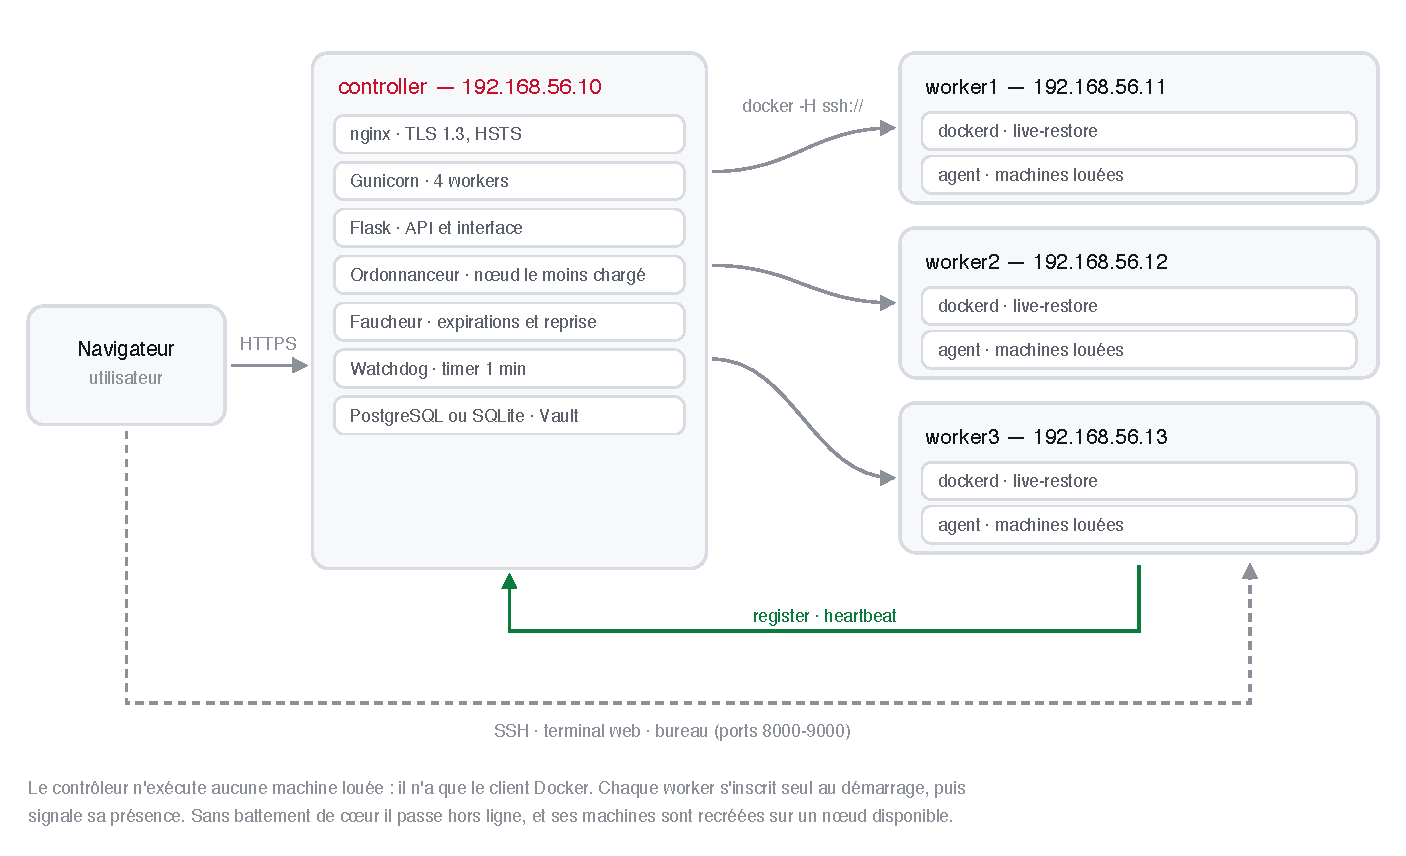
\includegraphics[width=0.95\textwidth]{figures/architecture.pdf}
\vspace{0.9cm}

\begin{minipage}{0.88\textwidth}
\color{gristexte}\small
Ce document explique \emph{tout} un projet réel : une plateforme qui loue des
machines Linux à la minute, accessibles en SSH, en terminal web ou en bureau
graphique dans le navigateur. On y part des notions --- qu'est-ce qu'un
conteneur, pourquoi un proxy inverse, ce que veut dire « idempotent » --- pour
arriver au code exact qui tourne en production.
\end{minipage}

\vfill
{\color{gristexte}\small
Projet 3 --- \textit{Outils de déploiement de plateformes}\\
INSA Centre-Val de Loire, STI 4A FISE, 2026/2027 --- Dr.~Nadia Fettah\\[6pt]
\today\par}
\end{titlepage}

% --- Sommaire ----------------------------------------------------------------
\pagenumbering{roman}
\setcounter{tocdepth}{1}
\tableofcontents
\cleardoublepage
\pagenumbering{arabic}

\chapter*{Avant-propos}
\addcontentsline{toc}{chapter}{Avant-propos}
\markboth{AVANT-PROPOS}{}

\section*{Ce que vous allez comprendre}

Un utilisateur arrive sur un site web, crée un compte, choisit « Ubuntu, bureau
graphique, 30 minutes », clique. Quinze secondes plus tard il a une machine
Linux à lui, avec une adresse SSH, un terminal dans son navigateur et un bureau
XFCE complet. Trente minutes plus tard, la machine a disparu toute seule et le
port qu'elle occupait est rendu.

Derrière ce clic, il y a un serveur web, une base de données, un démon Docker
sur trois machines différentes, un ordonnanceur qui choisit laquelle, un
service qui surveille les horloges, des certificats, un pare-feu, un coffre à
secrets, et une chaîne d'intégration qui refuse de publier quoi que ce soit
tant que onze contrôles ne sont pas au vert.

Ce document explique chacune de ces pièces. Pas en survol : le code exact, les
raisons de chaque choix, et les erreurs commises en chemin.

\begin{retenir}
À la fin de ce guide, vous devez être capable de reconstruire un projet de ce
type sans le recopier. C'est pour cela que chaque chapitre explique d'abord
\emph{pourquoi} avant de montrer \emph{comment}.
\end{retenir}

\section*{À qui s'adresse ce guide}

À quelqu'un qui sait programmer un peu, qui a déjà vu une ligne de commande,
et qui n'a jamais construit d'infrastructure. Aucune connaissance préalable de
Docker, d'Ansible, de Vagrant, de Flask ou de la sécurité web n'est supposée.

Chaque notion nouvelle est introduite dans un encadré bleu avant d'être
utilisée. Les pièges réellement rencontrés sont signalés en orange. Les points
à retenir sont en vert.

\begin{notion}{Comment lire les extraits de code}
Les extraits sont tirés du dépôt réel, sans retouche. Quand un fichier est trop
long pour tenir ici, seules les lignes qui portent l'idée sont reproduites et
les coupures sont marquées. Le chemin du fichier est toujours donné : vous
pouvez ouvrir l'original pour voir le reste.
\end{notion}

\section*{Le résultat, en images}

Avant de plonger dans la mécanique, voici ce que l'utilisateur voit.

\begin{figure}[htbp]
\centering
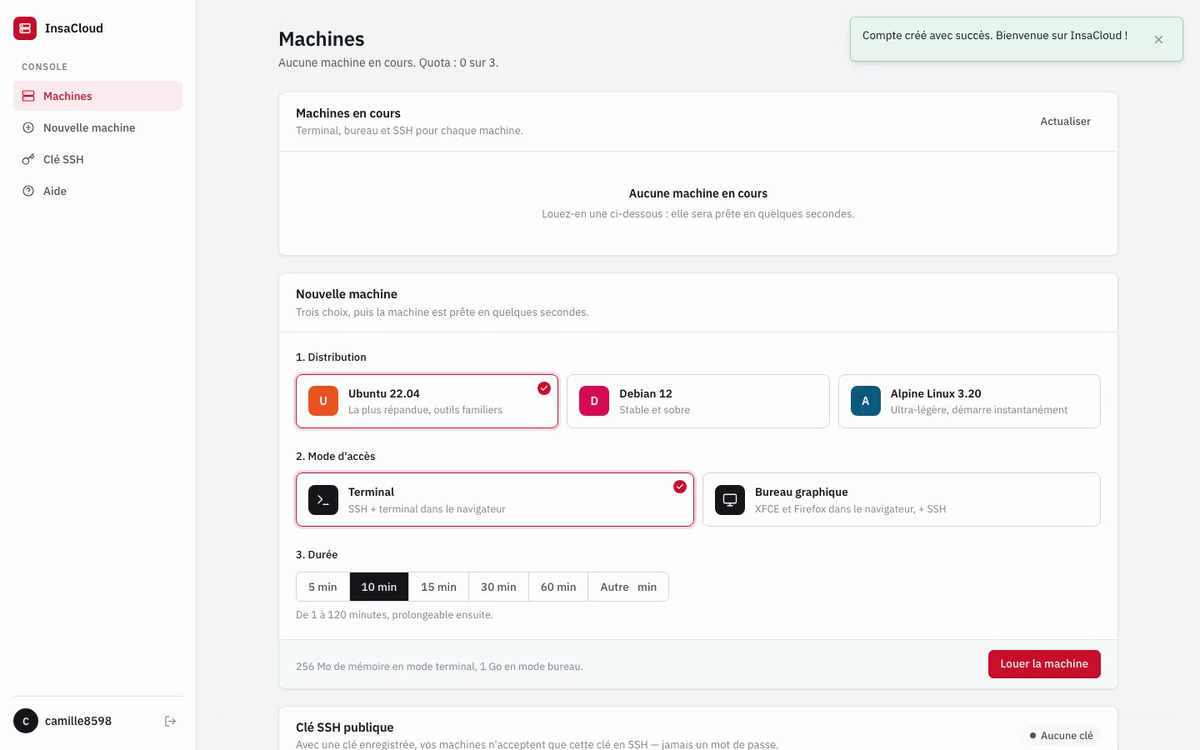
\includegraphics[width=0.78\textwidth]{../docs/03-tableau-de-bord.png}
\caption{Le tableau de bord. Les machines en cours, leur temps restant, et le
formulaire de location. Tout tient sur une page : c'est un choix, pas une
limite.}
\end{figure}

\begin{figure}[htbp]
\centering
\begin{minipage}{0.48\textwidth}
  \centering
  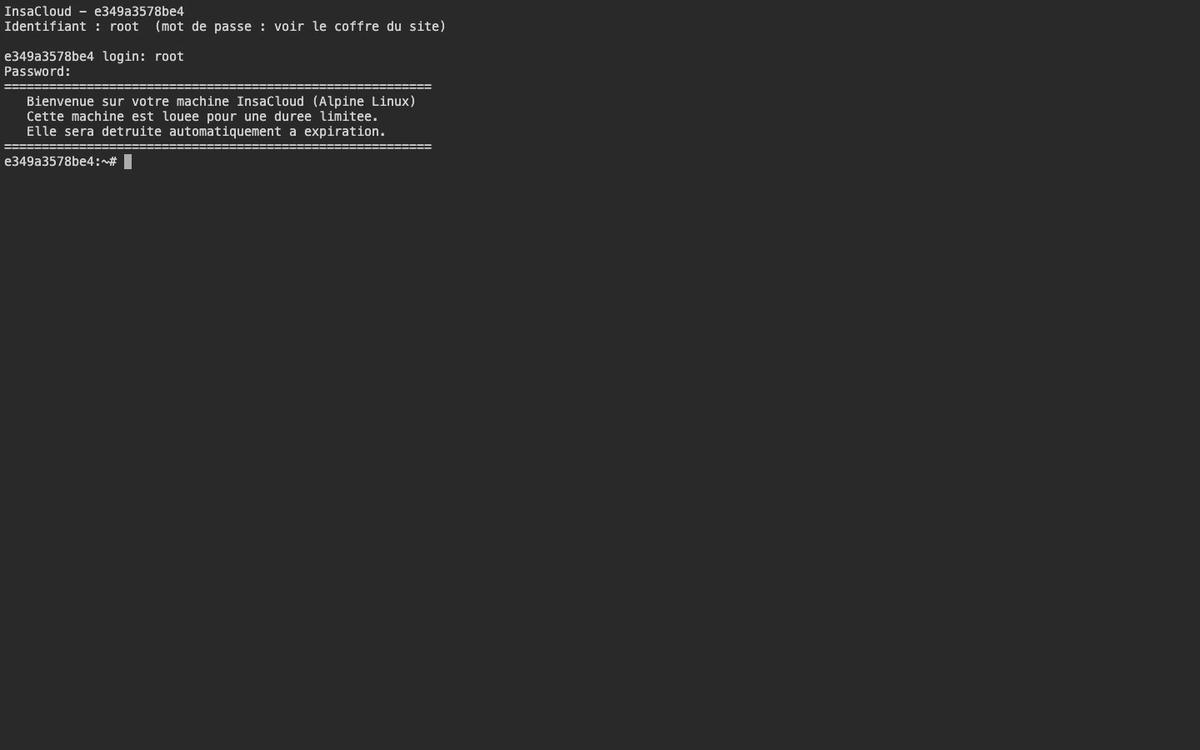
\includegraphics[width=\textwidth]{../docs/07-terminal-web.png}
\end{minipage}\hfill
\begin{minipage}{0.48\textwidth}
  \centering
  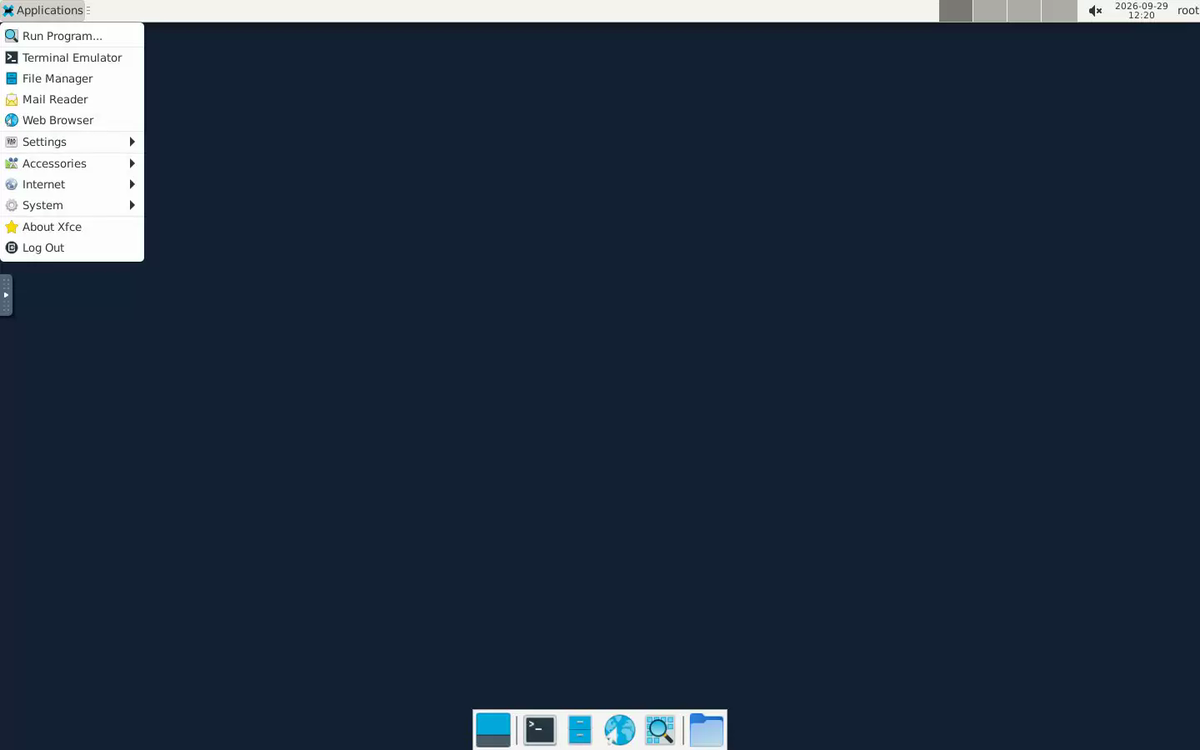
\includegraphics[width=\textwidth]{../docs/09-bureau-applications.png}
\end{minipage}
\caption{À gauche, un terminal dans le navigateur, sans rien installer. À
droite, un bureau XFCE complet avec Firefox, également dans le navigateur. La
même machine peut offrir l'un ou l'autre selon le mode choisi à la location.}
\end{figure}

\section*{Comment ce guide est organisé}

\begin{description}
\item[Partie I — Les notions] Ce qu'il faut savoir avant d'ouvrir le code :
  virtualisation, conteneurs, modèle web, infrastructure décrite en fichiers,
  et ce que « DevSecOps » veut dire concrètement.
\item[Partie II — L'architecture] La carte du territoire : qui parle à qui, où
  vivent les données, comment une machine naît et meurt.
\item[Partie III — La construction] Le cœur du guide. Chaque composant, son
  code, et les décisions qui l'ont façonné.
\item[Partie IV — Le déploiement] Comment tout cela arrive sur de vraies
  machines, en une commande, de façon reproductible.
\item[Partie V — La vérification] Les tests, la chaîne d'intégration, et le
  récit des défauts trouvés en faisant tourner le projet plutôt qu'en le
  relisant.
\item[Annexes] Commandes utiles, glossaire, erreurs fréquentes, et la grille de
  conformité au cahier des charges.
\end{description}

\section*{Le dépôt}

Tout le code commenté ici est public :
\url{https://github.com/aziz3r/insacloud}. Les chemins de fichiers mentionnés
dans le guide sont relatifs à la racine du dépôt.

\begin{center}
\begin{tabular}{@{}lr@{}}
\toprule
\textbf{Composant} & \textbf{Lignes} \\
\midrule
Application Flask (\fichier{2\_webapp/}) & environ 3\,500 \\
Tests (\fichier{2\_webapp/tests/}) & environ 1\,600 \\
Automatisation Ansible (\fichier{3\_ansible/}) & environ 1\,900 \\
Chaîne d'intégration (\fichier{.github/workflows/ci.yml}) & 601 \\
Images des machines (\fichier{1\_docker/}) & environ 400 \\
Infrastructure (\fichier{Vagrantfile}, \fichier{docker-compose.yml}) & 333 \\
\midrule
\textbf{Total} & \textbf{environ 10\,700} \\
\bottomrule
\end{tabular}
\end{center}

\part{Les notions}
\label{part:theorie}

\chapter{Le problème : louer des machines}

\section{Ce qu'on nous demande}

L'énoncé tient en une phrase : construire une plateforme où un utilisateur
s'inscrit, se connecte, loue une ou plusieurs instances Linux de différentes
distributions pour une durée qu'il choisit, y accède en SSH, et où le service
reste disponible même si une machine du parc tombe.

Derrière cette phrase se cachent dix-sept blocs de travail que le cahier des
charges détaille : l'environnement de développement, l'API web, la base de
données, la conteneurisation, l'infrastructure virtuelle, l'automatisation, un
agent sur chaque nœud, un ordonnanceur, le service de location, le déploiement
des conteneurs, l'accès SSH, l'expiration, la haute disponibilité, la sécurité,
la chaîne d'intégration, les tests, et la documentation.

\begin{notion}{Le vocabulaire du cloud}
Un \textbf{fournisseur de cloud} vend de la capacité de calcul à la demande. On
distingue trois niveaux de service :
\begin{description}
\item[IaaS] \emph{Infrastructure as a Service} --- on vous loue une machine
  nue, vous y installez ce que vous voulez. C'est Amazon EC2, et c'est ce que
  nous construisons.
\item[PaaS] \emph{Platform as a Service} --- on vous loue un endroit où
  déposer votre code, sans vous occuper de la machine. C'est Heroku.
\item[SaaS] \emph{Software as a Service} --- on vous loue un logiciel fini.
  C'est Gmail.
\end{description}
Notre plateforme est donc un mini-IaaS : l'utilisateur reçoit une machine et un
accès root dessus.
\end{notion}

\section{La décision qui structure tout : conteneurs plutôt que VM}

Louer « une machine Linux » peut se faire de deux façons.

\paragraph{Une machine virtuelle.} On émule un ordinateur entier : un noyau
Linux complet, son propre espace mémoire, ses disques virtuels. C'est ce que
fait VirtualBox ou VMware. L'isolation est quasi totale, mais démarrer une VM
prend trente secondes à une minute, et chacune réserve plusieurs centaines de
mégaoctets rien que pour son noyau.

\paragraph{Un conteneur.} On ne démarre pas de second noyau : on réutilise
celui de la machine hôte, en cloisonnant ce que le processus peut voir. Le
démarrage prend moins d'une seconde et le surcoût mémoire est celui des
processus eux-mêmes.

Pour une plateforme qui loue à la minute, la différence est décisive : un
utilisateur n'attend pas une minute après avoir cliqué. Le cahier des charges
tranche d'ailleurs explicitement --- « des conteneurs dans notre cas ».

\begin{figure}[htbp]
\centering
\resizebox{\textwidth}{!}{%
\begin{tikzpicture}[font=\small,
  bloc/.style={draw=grisligne,fill=grisfond,rounded corners=2pt,minimum height=7mm,
               align=center,inner sep=3pt},
  socle/.style={draw=grisligne,fill=white,rounded corners=2pt,minimum height=7mm,align=center}]

\node[font=\small\bfseries] at (2.6,5.1) {Machines virtuelles};
\node[socle,minimum width=5.2cm] at (2.6,0.0) {Matériel};
\node[socle,minimum width=5.2cm] at (2.6,0.8) {Système hôte};
\node[socle,minimum width=5.2cm] at (2.6,1.6) {Hyperviseur};
\foreach \x/\n in {0.95/1, 2.6/2, 4.25/3} {
  \node[bloc,minimum width=1.5cm] at (\x,2.5) {\scriptsize noyau invité};
  \node[bloc,minimum width=1.5cm] at (\x,3.3) {\scriptsize biblioth.};
  \node[bloc,minimum width=1.5cm,fill=bleufond] at (\x,4.1) {\scriptsize appli \n};
}
\draw[decorate,decoration={brace,amplitude=4pt},gristexte]
  (5.45,2.15) -- (5.45,4.45)
  node[midway,right=5pt,gristexte,font=\scriptsize,align=left]
  {chaque VM\\porte son\\propre noyau};

\node[font=\small\bfseries] at (11.2,5.1) {Conteneurs};
\node[socle,minimum width=5.2cm] at (11.2,0.0) {Matériel};
\node[socle,minimum width=5.2cm] at (11.2,0.8) {Système hôte --- \textbf{un seul noyau}};
\node[socle,minimum width=5.2cm] at (11.2,1.6) {Démon Docker};
\foreach \x/\n in {9.55/1, 11.2/2, 12.85/3} {
  \node[bloc,minimum width=1.5cm] at (\x,2.5) {\scriptsize biblioth.};
  \node[bloc,minimum width=1.5cm,fill=bleufond] at (\x,3.3) {\scriptsize appli \n};
}
\draw[decorate,decoration={brace,amplitude=4pt},vertok]
  (14.05,2.15) -- (14.05,3.65)
  node[midway,right=5pt,vertok,font=\scriptsize,align=left]
  {rien entre\\l'appli et le\\noyau de l'hôte};
\end{tikzpicture}}
\caption{La seule vraie différence : le conteneur n'embarque pas de noyau. Tout
le reste --- rapidité de démarrage, consommation mémoire, densité --- en
découle.}
\end{figure}

\begin{piege}{« Un conteneur, c'est une VM légère »}
C'est l'image qu'on donne souvent, et elle induit en erreur. Un conteneur
\emph{partage le noyau de l'hôte}. Conséquences concrètes :
\begin{itemize}
\item on ne peut pas faire tourner un conteneur Windows sur un noyau Linux ;
\item une faille d'évasion du noyau compromet l'hôte \emph{et} tous les autres
  conteneurs --- c'est pourquoi nous retirons les capacités Linux inutiles
  (chapitre~\ref{chap:securite}) ;
\item un conteneur n'a pas de \cmd{init} par défaut : pour y faire tourner
  plusieurs services, il faut en installer un (chapitre~\ref{chap:images}).
\end{itemize}
\end{piege}

\section{Les questions auxquelles il faut répondre}

Dire « on crée un conteneur par location » ne suffit pas. Il faut résoudre ce
que toute plateforme d'hébergement doit résoudre :

\begin{description}
\item[Où placer la machine ?] S'il y a trois serveurs, lequel choisir ? Que
  faire si l'un ne répond plus ?
\item[Comment y accéder ?] Un conteneur n'a pas d'adresse publique. Il faut
  publier un port, et deux machines ne peuvent pas prendre le même.
\item[Comment la faire disparaître ?] Personne ne viendra cliquer sur
  « supprimer » à 3 h du matin. Il faut un service qui surveille les horloges.
\item[Comment garder le secret ?] Le mot de passe root doit être montré à
  l'utilisateur, mais ne doit pas traîner en clair dans une base.
\item[Comment reconstruire tout cela ?] Si le serveur brûle, combien de temps
  faut-il pour remonter la plateforme à l'identique ?
\end{description}

Chacune occupe un chapitre de la partie~\ref{part:construction}.

\chapter{Conteneurs : ce qui se passe réellement}

\section{Trois mécanismes du noyau Linux}

Un conteneur n'est pas un objet du noyau. C'est un processus ordinaire auquel
on a appliqué trois mécanismes.

\begin{notion}{Les espaces de noms (\emph{namespaces})}
Un espace de noms cloisonne \emph{ce qu'un processus peut voir}. Linux en
propose plusieurs, dont :
\begin{description}
\item[PID] le processus se croit seul ; il voit son propre arbre de processus,
  numéroté à partir de 1.
\item[réseau] il a ses propres interfaces, sa table de routage, ses ports. Le
  port 22 du conteneur n'est pas le port 22 de l'hôte.
\item[montage] il a sa propre vision du système de fichiers.
\item[UTS] il a son propre nom de machine.
\end{description}
C'est l'illusion d'être seul au monde.
\end{notion}

\begin{notion}{Les groupes de contrôle (\emph{cgroups})}
Les espaces de noms cloisonnent la \emph{vue} ; les cgroups limitent la
\emph{consommation}. On y plafonne la mémoire, le temps processeur, le nombre
de processus, les entrées-sorties. Sans cgroups, un conteneur parti en boucle
infinie met à genoux tous les autres.

Dans notre projet, ces limites sont posées explicitement à la création :
\cmd{--memory}, \cmd{--memory-reservation}, \cmd{--cpus}, \cmd{--pids-limit}.
\end{notion}

\begin{notion}{Les capacités (\emph{capabilities})}
Historiquement, un processus était soit root (tout permis) soit non-root (rien).
Linux a découpé les pouvoirs de root en une quarantaine de \emph{capacités}
indépendantes : \cmd{CAP\_NET\_BIND\_SERVICE} (écouter sous le port 1024),
\cmd{CAP\_SYS\_ADMIN} (monter des systèmes de fichiers), etc.

On peut donc autoriser un processus à écouter sur le port 22 sans l'autoriser
à charger un module noyau. C'est exactement ce que fait notre durcissement :
retirer tout, puis rendre les dix capacités dont \cmd{sshd} a réellement
besoin.
\end{notion}

\section{Les images et le système de fichiers en couches}

Une \textbf{image} est un modèle figé, en lecture seule. Un \textbf{conteneur}
est une instance en exécution de cette image, avec une fine couche
inscriptible par-dessus.

\begin{figure}[htbp]
\centering
\begin{tikzpicture}[font=\small,
  couche/.style={draw=grisligne,fill=grisfond,minimum width=7.4cm,minimum height=8mm,
                 align=center,inner sep=2pt}]
\node[couche] at (0,0) {\texttt{\scriptsize FROM ubuntu:22.04}\quad\textcolor{gristexte}{\scriptsize 77 Mo}};
\node[couche] at (0,0.85) {\texttt{\scriptsize RUN apt-get install openssh-server ...}\quad\textcolor{gristexte}{\scriptsize 38 Mo}};
\node[couche] at (0,1.7) {\texttt{\scriptsize COPY entrypoint.sh}\quad\textcolor{gristexte}{\scriptsize 4 Ko}};
\node[couche,fill=bleufond,draw=bleutrait] at (0,2.75)
  {\scriptsize couche inscriptible du conteneur\quad\textcolor{bleutrait}{\scriptsize vide au départ}};
\draw[decorate,decoration={brace,amplitude=5pt},gristexte]
  (3.9,-0.42) -- (3.9,2.12)
  node[midway,right=6pt,gristexte,font=\scriptsize,align=left]
  {l'\textbf{image} :\\en lecture seule,\\partagée entre tous\\les conteneurs};
\draw[decorate,decoration={brace,amplitude=5pt},bleutrait]
  (3.9,2.35) -- (3.9,3.15)
  node[midway,right=6pt,bleutrait,font=\scriptsize,align=left]
  {le \textbf{conteneur} :\\jetable};
\end{tikzpicture}
\caption{Une image est un empilement de couches. Dix conteneurs issus de la
même image ne stockent la base qu'une fois : seule la couche du dessus leur est
propre.}
\end{figure}

Cette architecture a une conséquence qu'on oublie vite : \textbf{détruire un
conteneur détruit sa couche inscriptible}, donc tout ce que l'utilisateur y a
écrit. C'est pourquoi le projet sauvegarde le travail avant destruction
(chapitre~\ref{chap:archives}) et pourquoi la reprise après panne ne rend pas
les fichiers (chapitre~\ref{chap:ha}).

\begin{retenir}
Une image, c'est la recette figée. Un conteneur, c'est le plat : on le mange,
on jette l'assiette. Tout ce qui doit survivre est rangé ailleurs --- dans un
volume, dans une base, ou dans une archive.
\end{retenir}

\section{Les commandes qu'il faut connaître}

\begin{lstlisting}[language=bash]
# Construire une image a partir du Dockerfile du dossier courant
docker build -t mon_image:latest .

# Lancer un conteneur en arriere-plan (-d), en publiant un port
docker run -d --name ma_machine -p 2222:22 mon_image:latest

# Lister ce qui tourne ; -a ajoute ce qui est arrete
docker ps
docker ps -a --filter "label=insacloud.role=rented-machine"

# Entrer dans un conteneur qui tourne
docker exec -it ma_machine /bin/bash

# Comprendre pourquoi il ne demarre pas
docker logs ma_machine

# Tout savoir de sa configuration reelle (ports, limites, capacites)
docker inspect ma_machine

# Le detruire, meme s'il tourne
docker rm -f ma_machine
\end{lstlisting}

\begin{notion}{Publier un port}
\cmd{-p 2222:22} signifie : « ce qui arrive sur le port \textbf{2222 de
l'hôte} est transmis au port \textbf{22 du conteneur} ». Le conteneur croit
écouter sur 22 ; le monde extérieur frappe sur 2222.

C'est le mécanisme qui permet de faire tourner cent serveurs SSH sur une seule
machine : chacun écoute son 22 interne, mais reçoit un port externe différent.
Notre plateforme en attribue un dans la plage 8000--9000 et garantit l'unicité
par un index en base (chapitre~\ref{chap:bdd}).
\end{notion}

\chapter{Une application web, de bout en bout}

\section{Ce qui se passe quand on tape une adresse}

\begin{figure}[htbp]
\centering
\resizebox{\textwidth}{!}{%
\begin{tikzpicture}[font=\scriptsize,
  b/.style={draw=grisligne,fill=grisfond,rounded corners=2pt,minimum height=12mm,
            minimum width=2.1cm,align=center},
  f/.style={-{Stealth[length=2mm]},gristexte}]
\node[b] (nav) at (0,0) {Navigateur\\\textcolor{gristexte}{Firefox}};
\node[b] (ngx) at (3,0) {nginx\\\textcolor{gristexte}{port 443}};
\node[b] (gun) at (6,0) {Gunicorn\\\textcolor{gristexte}{port 5000}};
\node[b] (fl) at (9,0) {Flask\\\textcolor{gristexte}{votre code}};
\node[b] (db) at (12,0) {PostgreSQL\\\textcolor{gristexte}{port 5432}};
\draw[f] (nav) -- node[above]{HTTPS} (ngx);
\draw[f] (ngx) -- node[above]{HTTP} node[below]{local} (gun);
\draw[f] (gun) -- node[above]{WSGI} (fl);
\draw[f] (fl) -- node[above]{SQL} (db);
\draw[{Stealth[length=2mm]}-,gristexte,dashed] (nav.south) ++(0,-0.5)
  -- ++(12,0) node[midway,below,gristexte]{la réponse repart par le même chemin};
\draw[gristexte,dashed] (db.south) -- ++(0,-0.5);
\end{tikzpicture}}
\caption{La chaîne complète d'une requête. Chaque maillon a une raison d'être
précise.}
\end{figure}

\paragraph{Pourquoi nginx devant ?} Flask sait répondre à du HTTP, mais n'est
pas prévu pour affronter Internet. On place donc un \emph{proxy inverse}
devant : nginx termine le TLS (le « s » de HTTPS), sert les fichiers statiques
--- images, CSS --- sans réveiller Python, impose des en-têtes de sécurité, et
protège l'application des requêtes malformées.

\begin{notion}{Proxy direct et proxy inverse}
Un \textbf{proxy direct} agit pour le client : votre navigateur passe par lui
pour atteindre le web. Un \textbf{proxy inverse} agit pour le serveur : le
client croit parler au site, alors qu'il parle à nginx, qui relaie. Le premier
cache qui demande, le second cache qui répond.
\end{notion}

\paragraph{Pourquoi Gunicorn ?} Le serveur de développement de Flask traite une
requête à la fois et le dit lui-même : « ne pas utiliser en production ».
Gunicorn lance plusieurs processus ouvriers qui se partagent les requêtes,
redémarre ceux qui plantent, et sait s'arrêter proprement.

\begin{notion}{WSGI}
\emph{Web Server Gateway Interface} est le contrat entre un serveur Python et
une application Python. L'application expose un objet appelable qui reçoit un
dictionnaire décrivant la requête et renvoie une réponse. Grâce à ce contrat,
on remplace Gunicorn par uWSGI ou Waitress sans toucher une ligne de Flask.
\end{notion}

\begin{piege}{Un seul processus Gunicorn n'est pas une option}
Avec un seul ouvrier, une requête lente --- créer un conteneur prend plusieurs
secondes --- bloque \emph{tous} les autres utilisateurs. Notre déploiement en
lance quatre. Mais plusieurs processus qui démarrent simultanément posent un
autre problème, celui de la course à l'initialisation de la base : nous y
revenons au chapitre~\ref{chap:bdd}, car il nous a réellement coûté une panne.
\end{piege}

\section{Flask en dix minutes}

Flask est un \emph{micro}-framework : il fournit le routage, les gabarits et
les sessions, et laisse le reste à des bibliothèques que vous choisissez. C'est
l'inverse de Django, qui décide à votre place.

\begin{lstlisting}[language=Python]
from flask import Flask, render_template, request, redirect, url_for, session

app = Flask(__name__)
app.secret_key = "..."           # sert a SIGNER les cookies de session

@app.route("/")                  # une URL ...
def accueil():                   # ... associee a une fonction
    return render_template("index.html", titre="Bonjour")

@app.route("/login", methods=["GET", "POST"])
def login():
    if request.method == "POST":
        session["user"] = request.form["username"]   # cookie signe
        return redirect(url_for("accueil"))
    return render_template("login.html")
\end{lstlisting}

\begin{description}
\item[Le routage] \cmd{@app.route} associe un chemin d'URL à une fonction. La
  fonction renvoie ce que le navigateur recevra.
\item[Les gabarits] \cmd{render\_template} remplit un fichier HTML avec des
  variables, grâce au moteur Jinja2.
\item[La session] \cmd{session} est un dictionnaire stocké \emph{dans un
  cookie} chez le client.
\end{description}

\begin{piege}{Une session Flask est signée, pas chiffrée}
C'est l'erreur la plus courante, et nous l'avons commise. Le contenu d'un
cookie de session est encodé en base64 : \textbf{n'importe qui peut le lire},
sans la clé. La signature empêche seulement de le \emph{modifier}.

Nous y avions mis le mot de passe root d'une machine, le temps de l'afficher
une fois. Il suffisait d'ouvrir les outils du navigateur pour le récupérer. La
correction consiste à ne stocker que l'identifiant de la machine et à relire le
secret en base, chiffré (chapitre~\ref{chap:securite}).
\end{piege}

\section{Le même chemin pour un humain et pour un programme}

Un trait d'architecture qui revient partout dans ce projet : chaque route sert
soit du HTML, soit du JSON, selon ce que l'appelant demande dans l'en-tête
\cmd{Accept}. Il n'y a donc pas un site d'un côté et une API de l'autre, mais
une seule logique métier avec deux rendus.

\begin{lstlisting}[language=Python,caption={\fichier{2\_webapp/app.py} --- choisir le format de la réponse}]
def veut_json() -> bool:
    # Un client qui accepte TOUT (Accept: */*, cas de curl sans en-tete)
    # n'est pas un client d'API : seul celui qui demande du JSON sans accepter
    # le HTML est traite comme tel.
    accepte = request.accept_mimetypes
    return accepte.accept_json and not accepte.accept_html
\end{lstlisting}

\begin{piege}{\texttt{Accept: */*} n'est pas une demande de JSON}
Notre première version répondait du JSON à tout client acceptant
\cmd{application/json} --- ce que fait \cmd{*/*}. Résultat : certains
navigateurs et tous les \cmd{curl} nus recevaient du JSON à la place de la
page. La condition correcte est : \emph{accepte le JSON} \textbf{et}
\emph{n'accepte pas le HTML}.
\end{piege}

\chapter{L'infrastructure décrite dans des fichiers}

\section{Le problème du « ça marche chez moi »}

Un projet installé à la main sur un serveur a une propriété désastreuse :
personne, pas même son auteur, ne sait exactement ce qui a été fait. Au
remontage, il manque toujours un paquet, un fichier de configuration, une
permission.

L'\emph{infrastructure as code} consiste à écrire l'état voulu dans des
fichiers versionnés, et à laisser un outil l'appliquer. Deux outils se
partagent le travail.

\begin{description}
\item[Vagrant] crée les machines virtuelles : combien, à partir de quelle
  image, avec quelle mémoire, quelle adresse.
\item[Ansible] les configure : installe les paquets, dépose les fichiers,
  démarre les services.
\end{description}

\section{Vagrant : des VM reproductibles}

\begin{lstlisting}[language=Ruby,caption={Le principe, en quelques lignes}]
Vagrant.configure("2") do |config|
  config.vm.box = "bento/ubuntu-22.04"       # l'image de base
  config.vm.define "worker1" do |node|
    node.vm.hostname = "worker1"
    node.vm.network "private_network", ip: "192.168.56.11"
    node.vm.provider "virtualbox" do |v|
      v.memory = 3072
      v.cpus   = 2
    end
  end
end
\end{lstlisting}

\cmd{vagrant up} lit ce fichier et crée la VM ; \cmd{vagrant destroy} l'efface.
Entre les deux, l'état est entièrement décrit par le fichier : n'importe qui,
sur n'importe quelle machine, obtient le même résultat.

\begin{notion}{\emph{Box} et \emph{provider}}
Une \textbf{box} est une image de VM préfabriquée, téléchargée depuis un
catalogue public. Un \textbf{provider} est le logiciel de virtualisation qui
l'exécute : VirtualBox, VMware, Parallels, QEMU. Le même \cmd{Vagrantfile} peut
cibler plusieurs providers --- indispensable ici, car VirtualBox ne fonctionne
pas sur les Mac à puce Apple.
\end{notion}

\section{Ansible : décrire l'état, pas les étapes}

Ansible se connecte en SSH et applique des \emph{tâches}. La différence avec un
script shell est fondamentale.

\begin{lstlisting}[language=bash,caption={Un script shell décrit des actions}]
apt-get install -y nginx          # se comporte mal si deja installe
mkdir /etc/insacloud              # echoue si le dossier existe
echo "..." > /etc/insacloud/conf  # ecrase a chaque fois
systemctl restart nginx           # redemarre meme si rien n'a change
\end{lstlisting}

\begin{lstlisting}[language=yamlplus,caption={Ansible décrit un état voulu}]
- name: nginx est installe
  ansible.builtin.apt:
    name: nginx
    state: present

- name: Le dossier de configuration existe, avec les bons droits
  ansible.builtin.file:
    path: /etc/insacloud
    state: directory
    owner: insacloud
    mode: "0750"

- name: La configuration est en place
  ansible.builtin.template:
    src: insacloud.conf.j2
    dest: /etc/insacloud/conf
  notify: Redemarrer nginx        # UNIQUEMENT si le fichier a change
\end{lstlisting}

\begin{notion}{Idempotence}
Une opération est \textbf{idempotente} si l'appliquer deux fois donne le même
résultat que l'appliquer une fois. C'est la propriété centrale d'Ansible :
relancer le playbook sur un serveur déjà configuré ne doit \emph{rien} changer.

La preuve se lit dans le compte rendu : au second passage, \cmd{changed=0}.
Dans ce projet, c'est mesuré sur les quatre nœuds à chaque modification
(chapitre~\ref{chap:ansible}).
\end{notion}

\begin{retenir}
Idempotent ne veut pas dire « ne fait rien la deuxième fois », mais « vérifie
l'état, et n'agit que s'il diffère de celui qui est voulu ». La nuance compte :
c'est elle qui permet de relancer le déploiement sans crainte, à n'importe quel
moment.
\end{retenir}

\paragraph{Le vocabulaire d'Ansible.}
\begin{description}
\item[Inventaire] la liste des machines, rangées par groupes
  (\cmd{[controllers]}, \cmd{[workers]}).
\item[Tâche] une action unitaire, exprimée par un \emph{module} :
  \cmd{apt}, \cmd{file}, \cmd{template}, \cmd{systemd}.
\item[Rôle] un ensemble de tâches réutilisable, avec ses variables par défaut,
  ses fichiers et ses gabarits. Le projet en compte neuf.
\item[Playbook] la partition : quels rôles sur quels groupes, dans quel ordre.
\item[Handler] une tâche qui ne s'exécute que si une autre a changé quelque
  chose. Typiquement : redémarrer un service.
\item[Vault] un fichier chiffré où ranger les secrets, versionnable sans
  danger.
\end{description}

\chapter{DevSecOps : pourquoi une chaîne automatique}

\section{Le constat}

Un projet d'école finit souvent par ne plus fonctionner que sur la machine de
son auteur, parce que rien ne vérifie le contraire. L'intégration continue
consiste à faire tourner, à chaque envoi de code, l'ensemble des contrôles que
personne n'a le courage de relancer à la main.

Le « Sec » de DevSecOps signifie que la sécurité fait partie de ces contrôles
automatiques, plutôt que d'être un audit ponctuel en fin de projet.

\section{Les familles de contrôles}

\begin{description}
\item[Lint] lit le code sans l'exécuter et signale ce qui est douteux :
  variable jamais utilisée, import mort, nom inconnu. Outils : \cmd{ruff} pour
  Python, \cmd{hadolint} pour les Dockerfiles, \cmd{ansible-lint}.
\item[Tests] exécutent le code sur des cas connus et comparent au résultat
  attendu. Outil : \cmd{pytest}.
\item[SAST] \emph{Static Application Security Testing} --- cherche des motifs
  dangereux dans le source : concaténation SQL, secret en dur, appel système
  construit à partir d'une entrée utilisateur. Outil : \cmd{bandit}.
\item[SCA] \emph{Software Composition Analysis} --- confronte la liste des
  dépendances aux bases de vulnérabilités publiques. Outil : \cmd{pip-audit}.
\item[Recherche de secrets] cherche clés et mots de passe commis par erreur,
  \emph{y compris dans l'historique} : effacer un secret dans un commit
  ultérieur ne l'efface pas du dépôt. Outil : \cmd{gitleaks}.
\item[DAST] \emph{Dynamic Application Security Testing} --- attaque
  l'application \emph{en fonctionnement} : en-têtes manquants, pages
  accessibles sans authentification, jetons CSRF absents. Outils : un script
  maison et \cmd{nuclei}.
\item[Scan d'image] cherche les CVE des paquets du système de base de l'image.
  Outil : \cmd{Trivy}.
\item[SBOM] \emph{Software Bill of Materials} --- l'inventaire exhaustif de ce
  qui est livré, conservé pour pouvoir répondre plus tard à « sommes-nous
  touchés par telle faille ? ». Outil : \cmd{Syft}.
\end{description}

\begin{figure}[htbp]
\centering
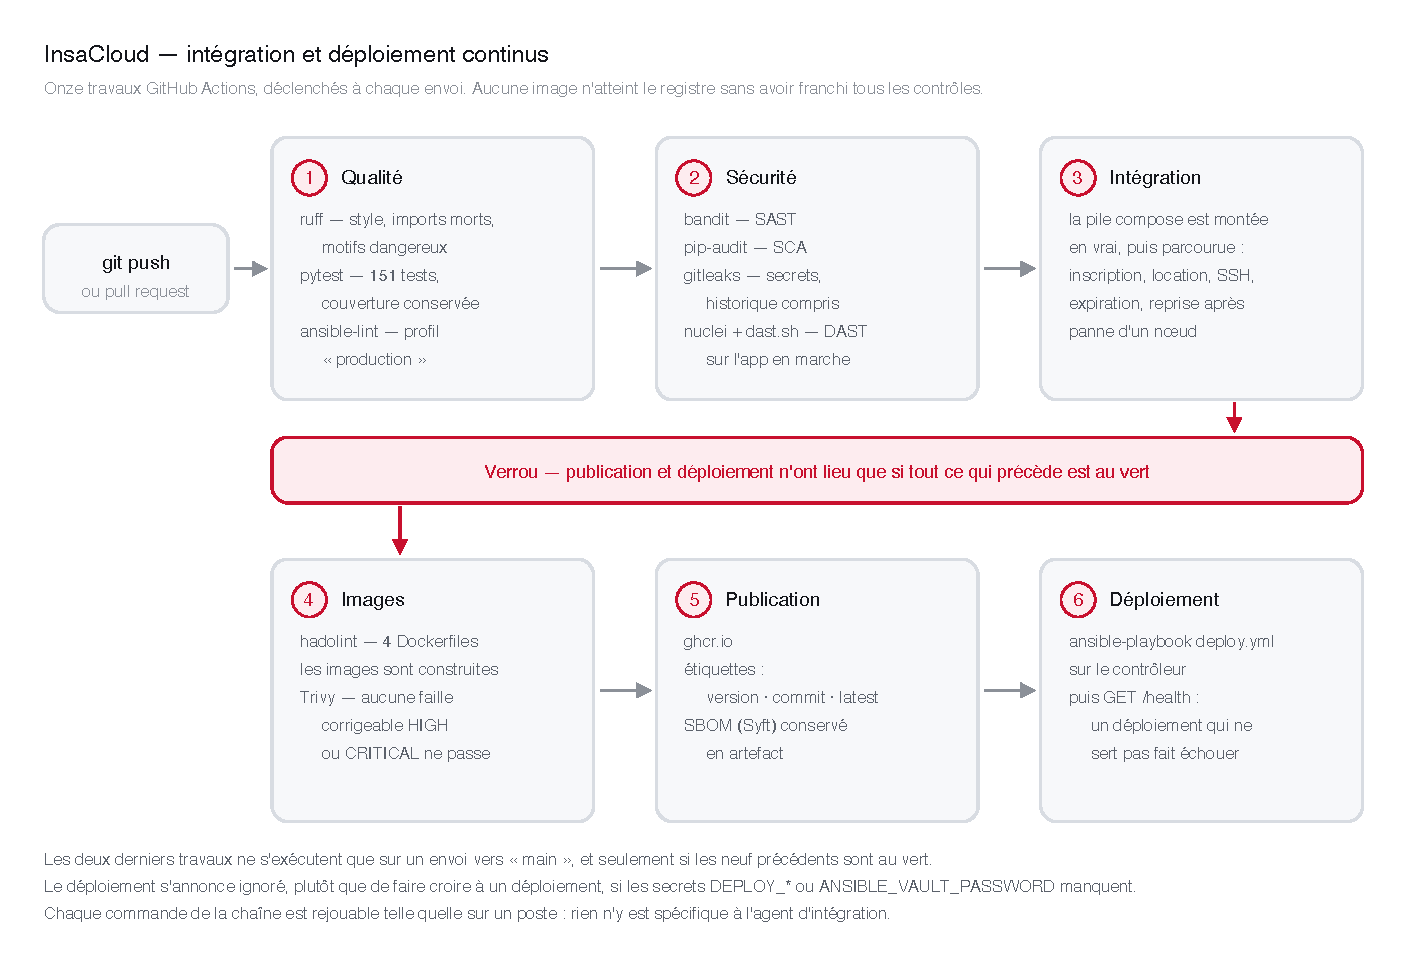
\includegraphics[width=\textwidth]{figures/chaine-ci-cd.pdf}
\caption{La chaîne réelle du projet : onze travaux, détaillés au
chapitre~\ref{chap:ci}.}
\end{figure}

\begin{notion}{CVE}
\emph{Common Vulnerabilities and Exposures} --- l'identifiant mondial unique
d'une faille connue, de la forme \cmd{CVE-2024-12345}. Les outils de SCA et de
scan d'image travaillent tous avec ces identifiants.
\end{notion}

\begin{retenir}
Une chaîne d'intégration n'est utile que si elle \emph{bloque}. Un contrôle qui
affiche un avertissement que personne ne lit ne sert à rien. Ici, aucune image
n'atteint le registre si l'un des contrôles échoue --- et c'est arrivé : nos
propres images ont été refusées par notre propre scan
(chapitre~\ref{chap:ci}).
\end{retenir}

\part{L'architecture}
\label{part:archi}

\chapter{La carte du territoire}

\section{Un contrôleur, trois exécutants}

\begin{figure}[htbp]
\centering
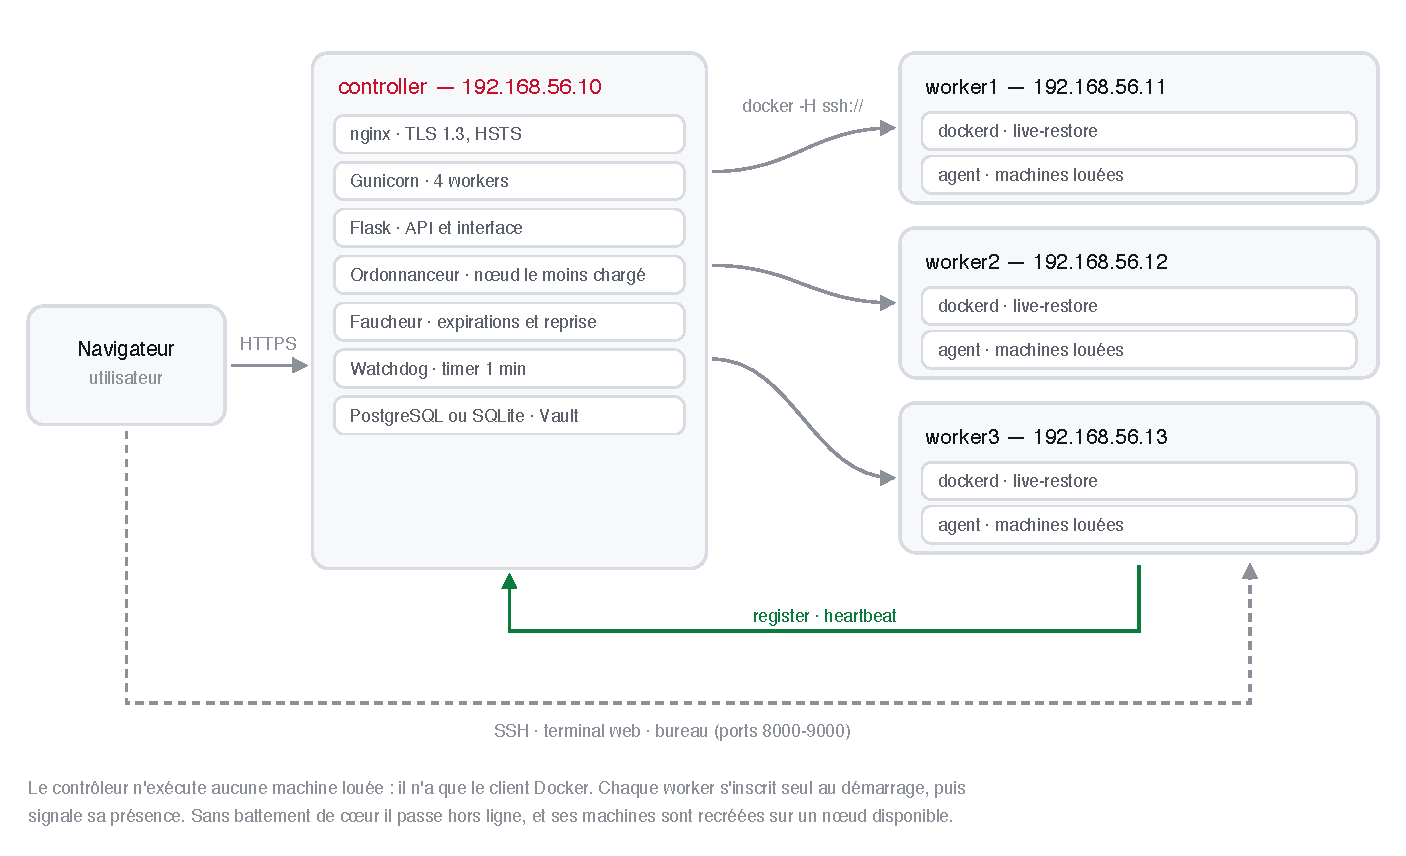
\includegraphics[width=\textwidth]{figures/architecture.pdf}
\caption{L'architecture déployée. Le contrôleur décide, les workers exécutent.}
\label{fig:archi}
\end{figure}

La plateforme se répartit sur quatre machines.

\paragraph{Le contrôleur} (192.168.56.10) porte tout ce qui réfléchit : le site
web, l'API, la base de données, l'ordonnanceur qui choisit où placer une
machine, et le Faucheur qui détruit celles qui ont expiré. Il n'exécute
\emph{aucune} machine louée et n'a même pas de démon Docker --- seulement le
client.

\paragraph{Les workers} (.11, .12, .13) portent tout ce qui exécute : un démon
Docker, les conteneurs loués, et un petit agent qui signale leur présence.

\begin{retenir}
Cette séparation n'est pas décorative. Elle garantit qu'un utilisateur qui
s'échapperait de son conteneur se retrouverait sur un worker --- une machine
sans base de données, sans clés, sans code de la plateforme. Le contrôleur,
lui, n'exécute rien qui vienne de l'extérieur.
\end{retenir}

\section{Comment le contrôleur pilote les workers}

Il existe deux façons de commander un démon Docker distant.

\paragraph{Exposer l'API Docker sur le réseau} (port 2375/2376). C'est simple,
et c'est une très mauvaise idée : qui parle au démon Docker d'une machine en
est root. Une erreur de pare-feu et toute la plateforme est compromise.

\paragraph{Passer par SSH.} Le client Docker sait le faire nativement :

\begin{lstlisting}[language=bash]
docker -H ssh://insacloud@worker1 ps
\end{lstlisting}

Aucun port Docker n'est ouvert. L'authentification est celle de SSH, par clé.
Le compte \cmd{insacloud} du worker n'a pas de mot de passe et n'est
joignable que depuis le contrôleur.

\begin{lstlisting}[language=Python,caption={\fichier{2\_webapp/workers.py} --- le préfixe de commande}]
def docker_command(worker: str = "local") -> list:
    """Prefixe de commande docker pour ce noeud."""
    host = worker_host(worker)
    if host is None:
        return ["docker"]
    return ["docker", "-H", f"ssh://{DOCKER_SSH_USER}@{host}"]
\end{lstlisting}

Toute commande Docker du projet passe par cette fonction. Conséquence
heureuse : le code est le même en mono-hôte (développement) et en cluster
(production). Seul le préfixe change.

\begin{notion}{Le mode mono-hôte}
Si l'inventaire ne déclare aucun worker, \cmd{worker\_host} renvoie
\cmd{None}, le préfixe se réduit à \cmd{docker}, et tout tourne sur la machine
locale. C'est ce qui permet de développer sur un portable sans monter quatre
VM, et c'est ce que fait la pile \cmd{docker compose}.
\end{notion}

\section{Comment le contrôleur apprend l'existence des workers}

C'est le point qui distingue une maquette d'une vraie plateforme :
\textbf{rien n'est écrit en dur}. Le contrôleur ne contient aucune liste
d'adresses de workers.

Chaque worker porte un petit agent qui, au démarrage, se présente au
contrôleur, puis signale régulièrement qu'il est toujours vivant.

\begin{figure}[htbp]
\centering
\begin{tikzpicture}[font=\scriptsize,
  b/.style={draw=grisligne,fill=grisfond,rounded corners=3pt,minimum height=8mm,
            minimum width=2.9cm,align=center},
  f/.style={-{Stealth[length=2mm]},vertok,thick}]
\draw[draw=grisligne,fill=white,rounded corners=4pt] (-1.75,-2.3) rectangle (1.75,2.1);
\node[font=\small\bfseries,insared] at (0,1.75) {contrôleur};
\node[b] at (0,1.0) {base de données};
\node[b] at (0,0.1) {API \texttt{/workers/*}};
\node[b] at (0,-0.8) {ordonnanceur};
\node[b] at (0,-1.7) {Faucheur};

\draw[draw=grisligne,fill=grisfond,rounded corners=4pt] (5.2,-0.85) rectangle (8.4,0.95);
\node[font=\small\bfseries] at (6.8,0.6) {worker2};
\node at (6.8,0.1) {agent};
\node[gristexte] at (6.8,-0.45) {dockerd};

\draw[f] (5.15,0.55) -- (1.85,0.55)
  node[midway,above,vertok]{1. \texttt{POST /workers/register}}
  node[midway,below,gristexte]{nom, IP, cœurs, mémoire};
\draw[f] (5.15,-0.2) -- (1.85,-0.2)
  node[midway,above,vertok]{2. \texttt{POST /workers/heartbeat}}
  node[midway,below,gristexte]{toutes les 30 s};
\draw[-{Stealth[length=2mm]},orangepartiel,thick,dashed] (1.85,-1.7) -- (5.15,-1.7)
  node[midway,above,orangepartiel,align=center]{3. plus de battement pendant 90 s};
\node[orangepartiel] at (6.8,-1.7) {OFFLINE};
\end{tikzpicture}
\caption{L'inscription spontanée. Allumer un worker suffit à l'ajouter au
parc ; l'éteindre suffit à l'en sortir.}
\end{figure}

\begin{retenir}
Ajouter un quatrième worker ne demande de modifier aucun fichier sur le
contrôleur. On l'allume, il s'inscrit, l'ordonnanceur commence à lui envoyer
des machines. C'est la \textbf{Fonctionnalité 7} du cahier des charges, et
c'est ce qui rend le parc élastique.
\end{retenir}

\chapter{Le modèle de données}
\label{chap:modele}

\begin{figure}[htbp]
\centering
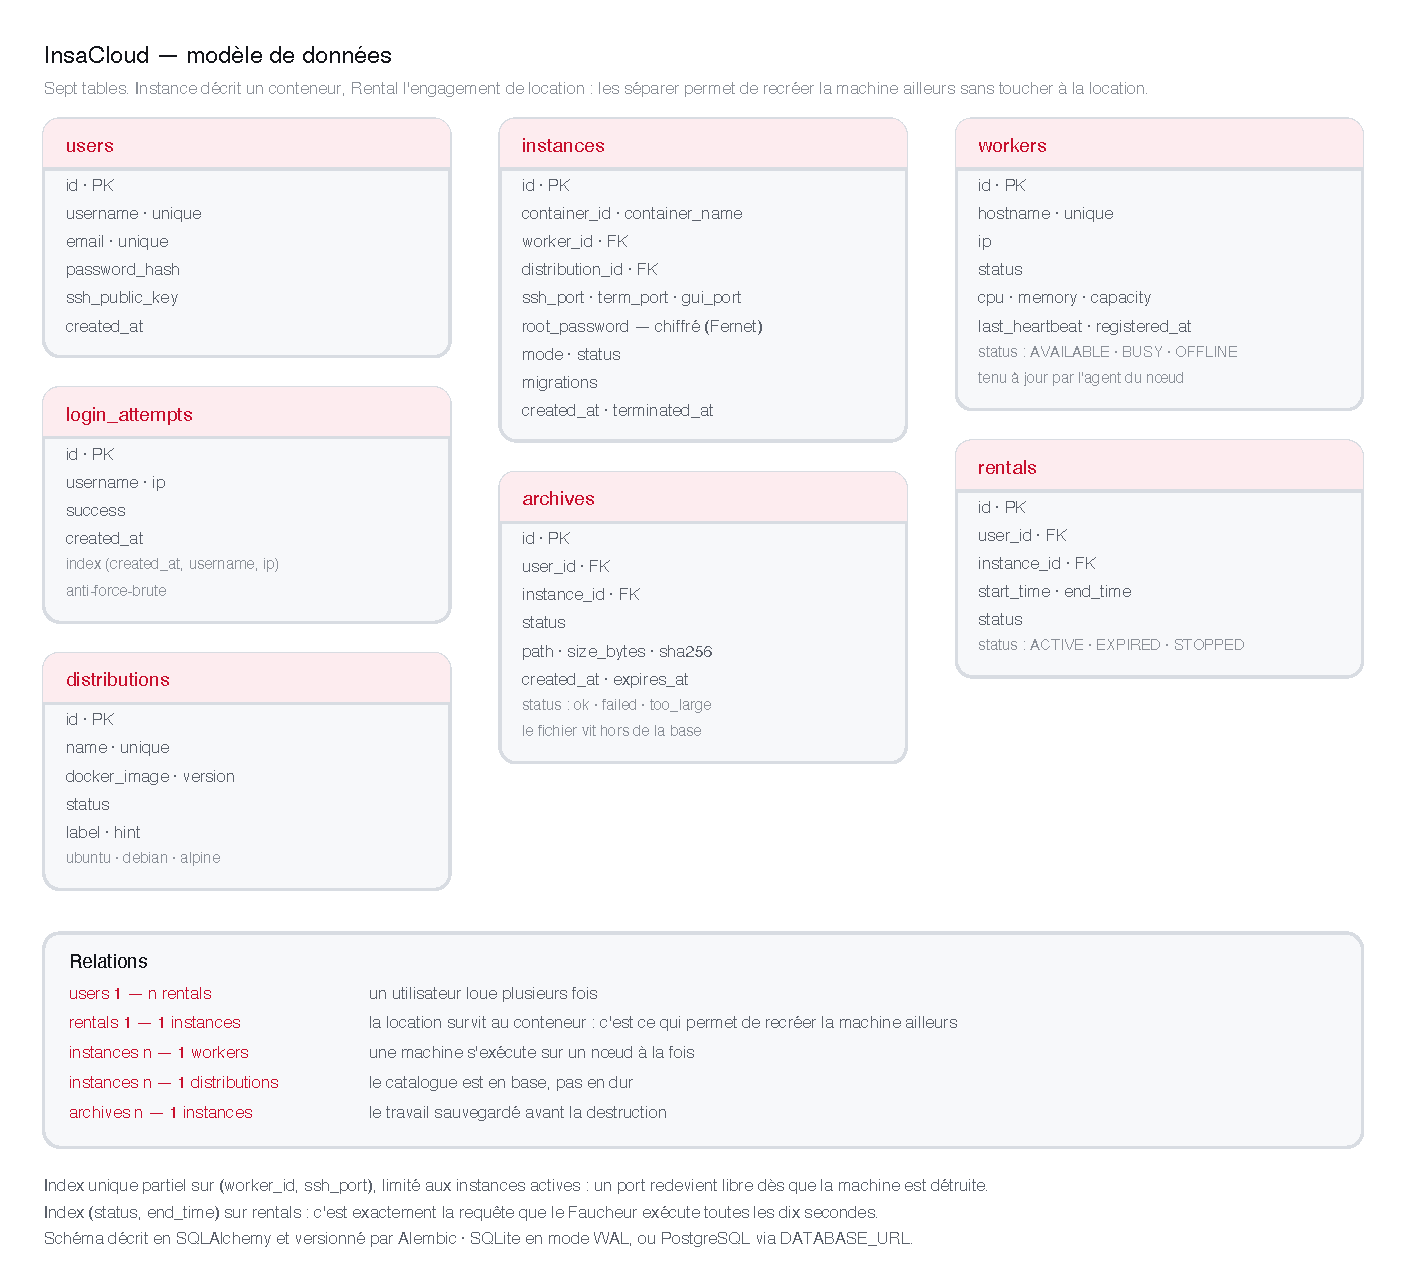
\includegraphics[width=\textwidth]{figures/base-de-donnees.pdf}
\caption{Les sept tables. La séparation \texttt{instances} / \texttt{rentals}
est la décision qui structure tout le reste.}
\label{fig:bdd}
\end{figure}

\section{Pourquoi séparer la machine de la location}

C'est le choix le moins évident et le plus important du projet.

On pourrait n'avoir qu'une table : une ligne par location, contenant à la fois
l'engagement (quel utilisateur, jusqu'à quand) et la machine (quel conteneur,
quel port, sur quel nœud). C'est plus court, et c'est ce qu'on écrit
naturellement.

Cela rend la reprise après panne \textbf{impossible}.

Quand un nœud tombe, il faut recréer la machine ailleurs : nouveau conteneur,
nouveau port, nouveau nœud, nouveau mot de passe. Mais la location, elle, ne
doit pas bouger : l'utilisateur a réservé trente minutes, il doit garder ses
trente minutes. Avec une table unique, on ne peut pas changer l'un sans
toucher à l'autre.

\begin{description}
\item[\texttt{Instance}] décrit un conteneur : son identifiant Docker, son
  nœud, ses ports, son mot de passe chiffré, son état.
\item[\texttt{Rental}] décrit l'engagement : quel utilisateur, de quand à
  quand, actif ou non.
\end{description}

La reprise change l'\texttt{Instance} et ne touche pas au \texttt{Rental}.

\begin{retenir}
Quand une table mélange « ce qui est promis » et « ce qui l'exécute », toute
panne devient visible par l'utilisateur. Séparer les deux est ce qui permet de
réparer sans rien lui reprendre.
\end{retenir}

\section{Les sept tables}

\begin{center}
\small
\begin{tabularx}{\textwidth}{@{}lX@{}}
\toprule
\textbf{Table} & \textbf{Ce qu'elle porte} \\
\midrule
\texttt{users} & comptes : identifiant, empreinte du mot de passe, clé SSH publique \\
\texttt{login\_attempts} & tentatives de connexion, pour le verrouillage anti-force-brute \\
\texttt{distributions} & le catalogue : Ubuntu, Debian, Alpine --- en base, pas en dur \\
\texttt{workers} & le parc : nom, adresse, état, charge, dernier battement de cœur \\
\texttt{instances} & les conteneurs : identifiant Docker, nœud, ports, secret chiffré \\
\texttt{rentals} & les locations : utilisateur, début, fin, état \\
\texttt{archives} & le travail sauvegardé avant destruction \\
\bottomrule
\end{tabularx}
\end{center}

\section{Deux index qui portent une règle métier}

Un index n'est pas qu'une optimisation : il peut imposer une contrainte que le
code aurait du mal à garantir seul.

\begin{lstlisting}[language=Python,caption={\fichier{2\_webapp/models.py} --- l'unicité du port}]
__table_args__ = (
    Index("idx_instances_status", "status"),
    # Index unique PARTIEL : deux machines actives ne peuvent pas partager un
    # port sur le meme noeud. La clause « where » le limite aux instances en
    # cours, donc un port redevient libre des que la machine est detruite.
    Index("uq_worker_port_actif", "worker_id", "ssh_port", unique=True,
          sqlite_where=text("status = 'running'"),
          postgresql_where=text("status = 'running'")),
)
\end{lstlisting}

\begin{notion}{Index unique partiel}
Un index unique classique interdirait deux fois le même port \emph{pour
toujours} : les machines détruites continueraient de réserver le leur. La
clause \cmd{WHERE} restreint la contrainte aux lignes qui comptent.

Sans cela, deux requêtes simultanées pourraient choisir le même port libre et
créer deux conteneurs en conflit --- une \emph{situation de compétition} que
le code applicatif ne peut pas écarter seul, car entre « ce port est libre »
et « je le prends » il s'écoule toujours un instant.
\end{notion}

Le second index sert le Faucheur :

\begin{lstlisting}[language=Python]
__table_args__ = (Index("idx_rentals_end", "status", "end_time"),)
\end{lstlisting}

C'est exactement la requête qu'il exécute toutes les dix secondes : « les
locations actives dont la date de fin est passée ». Sans index, chaque passage
relirait toute la table.

\chapter{Le cycle de vie d'une machine}
\label{chap:cycle}

\begin{figure}[htbp]
\centering
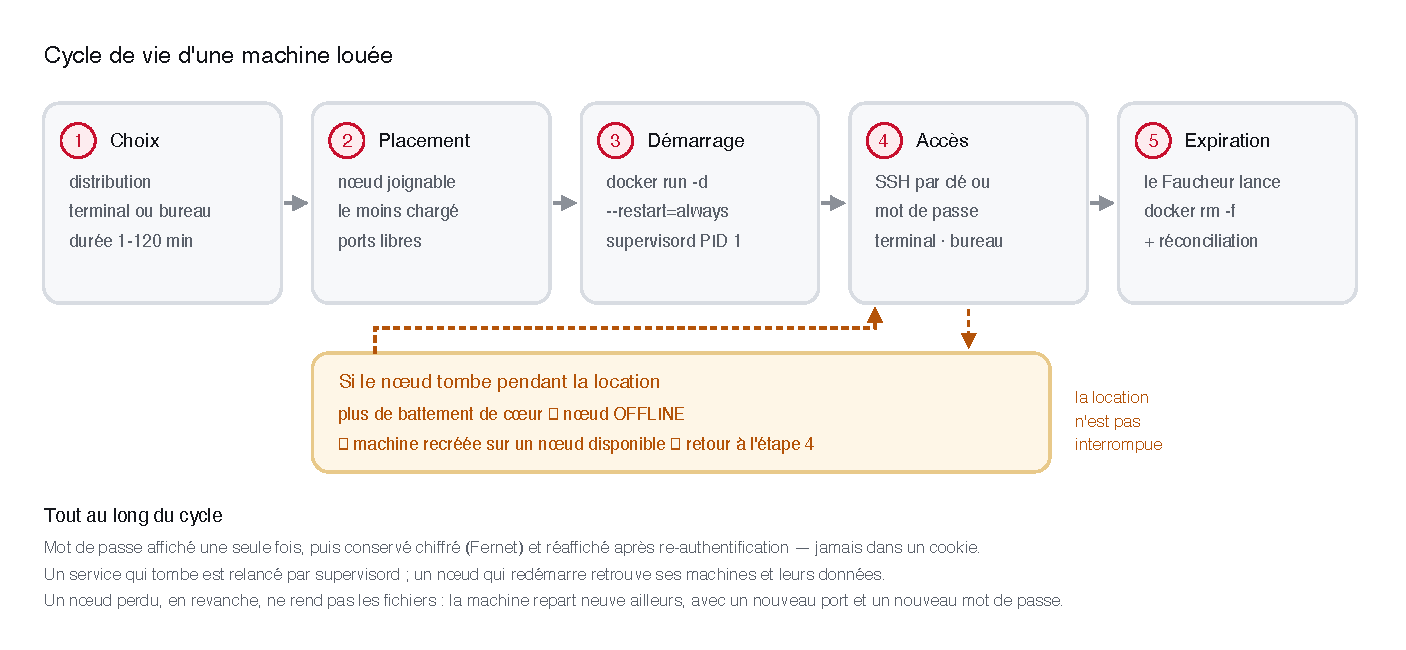
\includegraphics[width=\textwidth]{figures/cycle-de-vie.pdf}
\caption{De la demande à l'expiration, avec la branche de reprise si un nœud
tombe pendant la location.}
\label{fig:cycle}
\end{figure}

\section{Les cinq étapes}

\begin{enumerate}
\item \textbf{Choix.} L'utilisateur sélectionne une distribution, un mode
  (terminal ou bureau) et une durée de 1 à 120 minutes. Les trois valeurs sont
  validées côté serveur --- ce qui vient du navigateur n'est jamais cru.
\end{enumerate}

\begin{figure}[htbp]
\centering
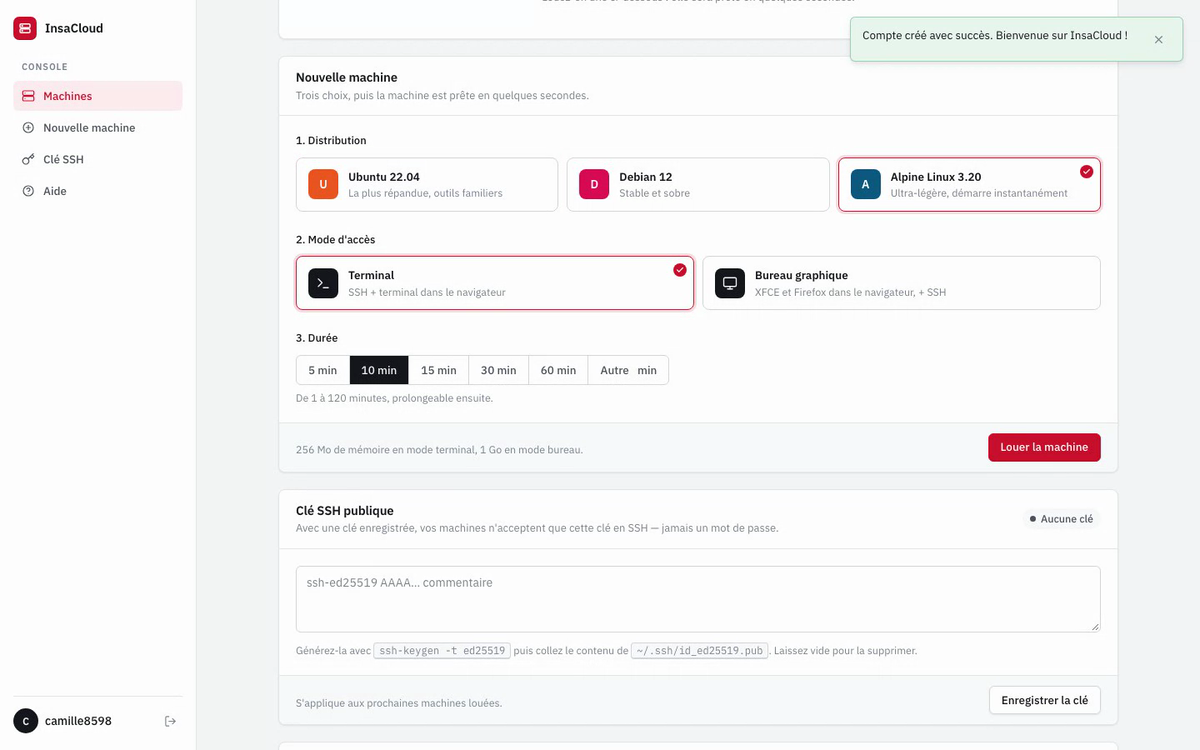
\includegraphics[width=0.84\textwidth]{../docs/04-choix-machine.png}
\caption{L'étape 1 vue par l'utilisateur. Une distribution dont l'image n'est
pas construite sur le parc n'apparaît pas : le catalogue interroge Docker
avant d'afficher un choix.}
\end{figure}

\begin{enumerate}
\setcounter{enumi}{1}
\item \textbf{Placement.} L'ordonnanceur retient le nœud joignable le moins
  chargé, puis réserve un port libre dans la plage 8000--9000.
\item \textbf{Démarrage.} \cmd{docker run -d --restart=always -p <port>:22}
  crée le conteneur ; \cmd{supervisord} y démarre en PID 1 et lance les
  services du mode choisi.
\item \textbf{Accès.} L'utilisateur reçoit une commande SSH et, selon le mode,
  l'adresse d'un terminal web ou d'un bureau. Le mot de passe root est affiché
  \emph{une seule fois}.
\item \textbf{Expiration.} Le Faucheur détruit la machine à l'échéance et
  libère le port.
\end{enumerate}

\section{La branche qui fait la différence}

Si le nœud tombe \emph{pendant} la location, l'agent cesse de battre. Au bout
de 90 secondes sans nouvelle, le contrôleur déclare le nœud hors ligne et
recrée ses machines sur un nœud disponible. L'utilisateur garde sa location,
sa durée et son droit d'accès ; il reçoit un nouveau port et un nouveau mot de
passe.

\begin{piege}{La reprise ne rend pas les fichiers}
Il faut le dire clairement, parce que c'est une limite assumée et pas un
oubli : les fichiers créés dans l'ancienne machine vivaient dans sa couche
inscriptible, sur un nœud devenu injoignable. Sans stockage partagé entre les
nœuds, ils sont perdus. Seul le \emph{service} repart.

Un volume répliqué (NFS, Ceph) changerait la nature du projet et son
périmètre. C'est un choix documenté, pas une négligence.
\end{piege}

\section{Trois niveaux de résilience}

La haute disponibilité se joue à trois échelles emboîtées, et c'est ce
qu'attend la \textbf{Fonctionnalité 13}.

\begin{center}
\small
\begin{tabularx}{\textwidth}{@{}llX@{}}
\toprule
\textbf{Échelle} & \textbf{Mécanisme} & \textbf{Ce qu'il rattrape} \\
\midrule
Dans la machine & \cmd{supervisord} & un service meurt (sshd, ttyd, VNC) : il est relancé \\
Sur le nœud & \cmd{--restart=always} & supervisord meurt : Docker relance le conteneur \\
Sur le nœud & \cmd{live-restore} & le démon Docker redémarre : les conteneurs continuent \\
Dans le parc & battement de cœur & le nœud entier tombe : les machines repartent ailleurs \\
\bottomrule
\end{tabularx}
\end{center}

\begin{figure}[htbp]
\centering
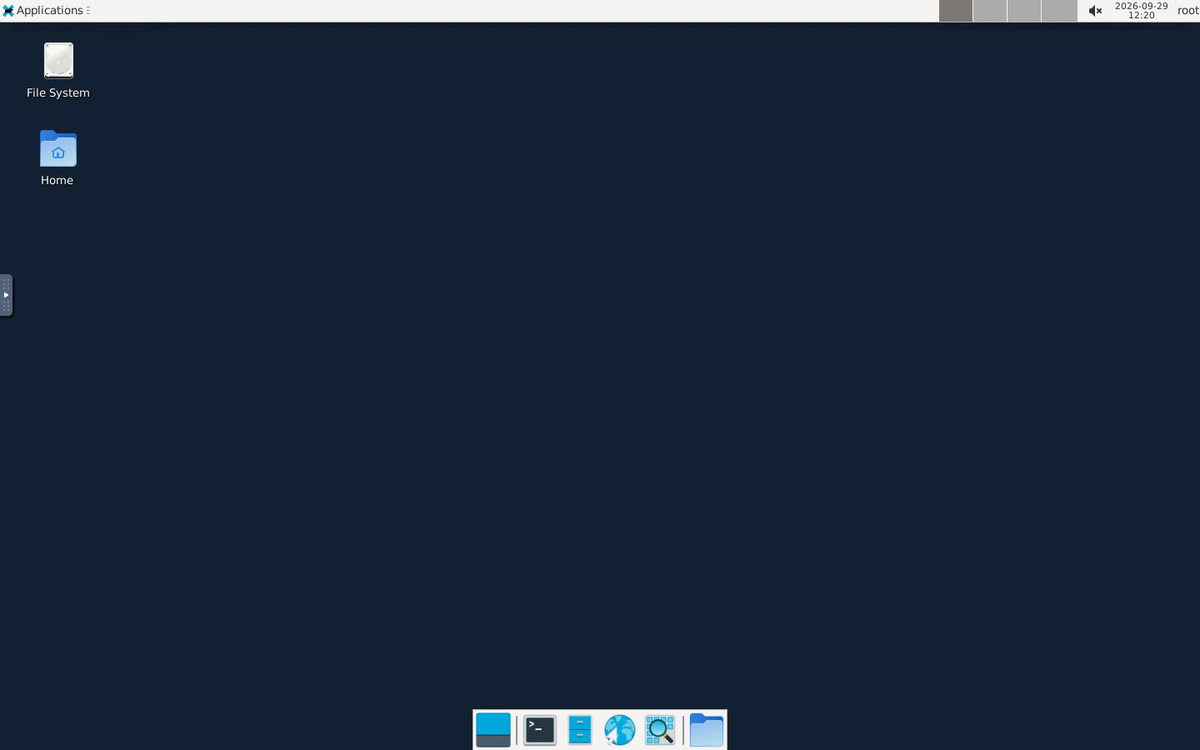
\includegraphics[width=0.84\textwidth]{../docs/10-machines-en-cours.png}
\caption{Deux machines en cours, une par mode d'accès. Le temps restant est
calculé à l'affichage ; c'est le Faucheur, et non la page, qui décide de la
destruction.}
\end{figure}

\begin{notion}{\texttt{live-restore}}
Par défaut, redémarrer le démon Docker arrête tous ses conteneurs. L'option
\cmd{live-restore} les laisse tourner pendant ce redémarrage. Pour une
plateforme de location, c'est la différence entre « une mise à jour de Docker
coupe tous les clients » et « personne ne s'en aperçoit ».
\end{notion}

\part{La construction}
\label{part:construction}

\chapter{Les images des machines louées}
\label{chap:images}

\section{Le problème : plusieurs services dans un conteneur}

Un conteneur exécute \emph{un} processus. Quand ce processus se termine, le
conteneur s'arrête. C'est voulu : un conteneur est censé faire une chose.

Or une machine louée doit en faire plusieurs à la fois : un serveur SSH, un
terminal web, et en mode bureau un serveur d'affichage, un gestionnaire de
fenêtres et une passerelle VNC vers le navigateur. Cinq processus.

Il faut donc un \emph{superviseur} : un processus qui démarre les autres, les
surveille, et relance celui qui meurt. Nous utilisons \cmd{supervisord}.

\begin{notion}{PID 1 et la responsabilité d'\emph{init}}
Le premier processus d'un espace de noms PID porte le numéro 1 et hérite d'une
obligation : adopter les processus orphelins et récupérer leur code de sortie.
Sans cela, les processus terminés s'accumulent à l'état \emph{zombie}.

Un \cmd{bash} lancé comme PID 1 ne fait pas ce travail. \cmd{supervisord}, si.
\end{notion}

\section{Trois Dockerfiles, six images}

Le projet propose trois distributions en deux modes. Plutôt que six fichiers,
on en écrit trois --- un par distribution --- et le mode devient un paramètre
de construction.

\begin{lstlisting}[language=dockerfile,caption={\fichier{1\_docker/Dockerfile} --- la structure (extraits)}]
FROM ubuntu:22.04

# DESKTOP=1 ajoute le serveur d'affichage, XFCE et noVNC.
ARG DESKTOP=0

RUN apt-get update \
    && apt-get install -y --no-install-recommends \
         openssh-server supervisor ca-certificates \
    && rm -rf /var/lib/apt/lists/*

# ... installation conditionnelle du bureau selon DESKTOP ...

COPY entrypoint.sh /usr/local/bin/entrypoint.sh
RUN chmod +x /usr/local/bin/entrypoint.sh

EXPOSE 22 7681 6080
CMD ["/usr/local/bin/entrypoint.sh"]
\end{lstlisting}

\begin{piege}{\texttt{apt-get install} sans nettoyage dans le même \texttt{RUN}}
Chaque instruction \cmd{RUN} crée une couche. Si l'on installe des paquets
dans une couche et qu'on efface le cache d'apt dans la couche
\emph{suivante}, le cache reste présent dans l'image : une couche ne peut pas
alléger celle du dessous.

Il faut donc enchaîner installation et nettoyage dans \emph{le même}
\cmd{RUN}, comme ci-dessus. Sur nos images, cela représente une cinquantaine
de mégaoctets.
\end{piege}

\begin{piege}{Un mot de passe par défaut dans l'image}
Notre première version contenait \cmd{ENV ROOT\_PASSWORD=insacloud}.
L'analyseur \cmd{hadolint} l'a signalé (règle DL3064), et il avait raison : ce
mot de passe aurait été le même sur \emph{toutes} les machines louées, et
visible par quiconque fait \cmd{docker history} sur l'image.

La correction : aucun mot de passe dans l'image. Si la plateforme n'en fournit
pas, l'entrypoint en tire un au hasard.
\end{piege}

\section{Le script de démarrage}

\begin{lstlisting}[language=bash,caption={\fichier{1\_docker/entrypoint.sh} --- le repli sûr}]
# Mot de passe root : fourni par la plateforme (-e ROOT_PASSWORD=...). S'il
# manque, on en tire un au hasard plutot que de retomber sur une valeur connue :
# un mot de passe par defaut serait le meme sur toutes les machines louees.
if [ -z "${ROOT_PASSWORD:-}" ]; then
    ROOT_PASSWORD="$(tr -dc 'A-Za-z2-9' < /dev/urandom | head -c 16)"
    echo "[insacloud] Aucun ROOT_PASSWORD fourni : tire au hasard = ${ROOT_PASSWORD}"
fi
\end{lstlisting}

Le script écrit ensuite une configuration \cmd{supervisord} adaptée au mode,
puis se remplace par le superviseur :

\begin{lstlisting}[language=bash]
exec "$(command -v supervisord)" -c "$CONF"
\end{lstlisting}

\begin{notion}{Pourquoi \texttt{exec}}
Sans \cmd{exec}, le shell resterait PID 1 et lancerait supervisord comme
enfant. Les signaux envoyés par Docker (\cmd{docker stop}) iraient au shell,
qui ne les relaierait pas : l'arrêt deviendrait brutal au bout du délai de
grâce.

\cmd{exec} remplace le processus courant : supervisord \emph{devient} le PID 1
et reçoit les signaux directement.
\end{notion}

\begin{figure}[htbp]
\centering
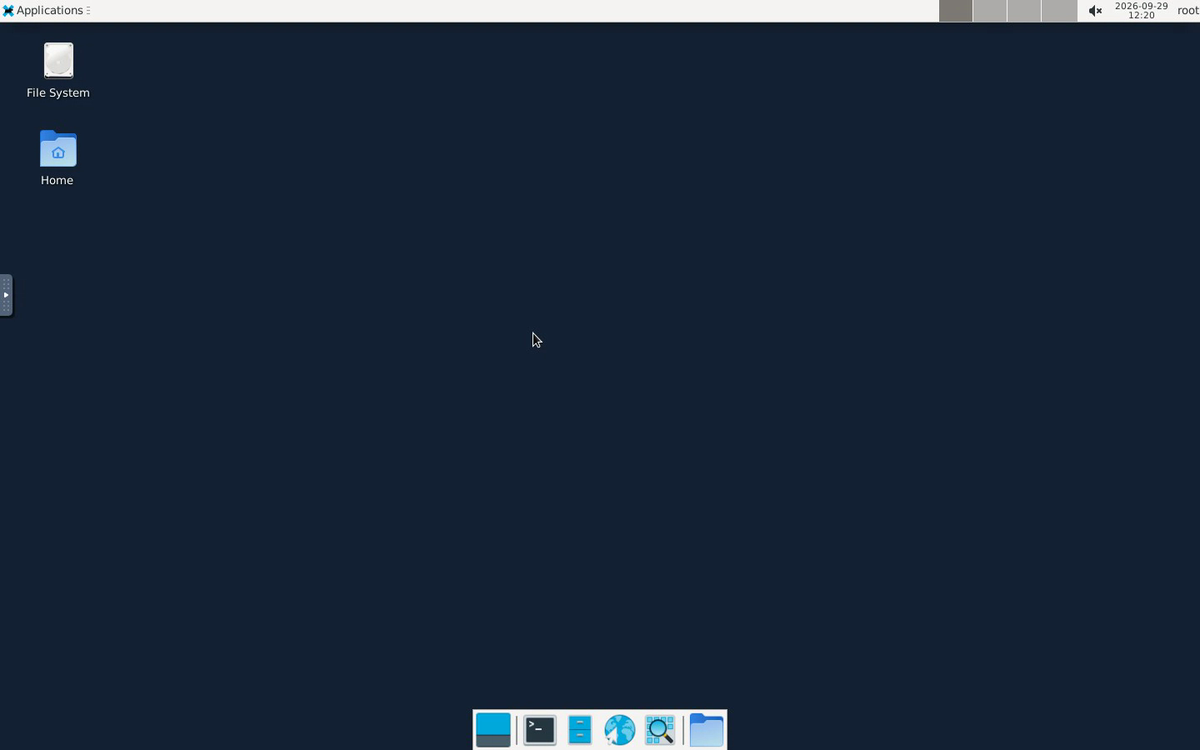
\includegraphics[width=0.78\textwidth]{../docs/08-bureau-xfce.png}
\caption{Le mode « bureau » : cinq processus cohabitent dans le conteneur ---
sshd, le terminal web, le serveur d'affichage, XFCE et la passerelle noVNC ---
tous surveillés par supervisord.}
\end{figure}

\section{Rotation du mot de passe à chaud}

L'utilisateur peut régénérer le mot de passe de sa machine sans la redémarrer.
Le même script sert de point d'entrée et d'outil :

\begin{lstlisting}[language=bash]
docker exec <conteneur> /usr/local/bin/entrypoint.sh setpass <nouveau>
\end{lstlisting}

SSH, terminal web et bureau prennent le nouveau mot de passe immédiatement.

\chapter{Piloter Docker depuis Python}

\section{Pourquoi la ligne de commande et pas un SDK}

Il existe une bibliothèque Python officielle (\cmd{docker-py}). Le cahier des
charges impose pourtant une commande précise :

\begin{center}
\cmd{docker run -d --restart=always -p <port>:22 <image>}
\end{center}

Piloter la CLI par \cmd{subprocess} rend cette commande \emph{visible dans le
code}. Chaque option passée se lit telle quelle. C'est un choix de lisibilité
et de conformité, pas une facilité.

\begin{lstlisting}[language=Python,caption={\fichier{2\_webapp/docker\_ops.py} --- l'appel central}]
def run_docker(*args, worker: str = "local", timeout: int = DOCKER_TIMEOUT) -> str:
    """Execute `docker <args>` sur le noeud `worker` (local ou distant via SSH)."""
    cmd = [*wk.docker_command(worker), *args]
    try:
        # Appel sans shell : les arguments sont passes en liste, donc jamais
        # re-interpretes par un interpreteur de commandes. Les seules valeurs
        # d'origine utilisateur (duree, distribution, mode) sont validees en amont.
        res = subprocess.run(cmd, capture_output=True, text=True, timeout=timeout)
    except FileNotFoundError as erreur:
        raise DockerError("La commande 'docker' est introuvable sur le serveur.") from erreur
    except subprocess.TimeoutExpired as erreur:
        raise DockerError("Docker n'a pas repondu dans le delai imparti.") from erreur
    if res.returncode != 0:
        message = res.stderr.strip() or f"docker {args[0]} a echoue ({res.returncode})"
        raise DockerError(message)
    return res.stdout.strip()
\end{lstlisting}

\begin{piege}{\texttt{shell=True} est une porte ouverte}
Écrire \cmd{subprocess.run(f"docker run ... \{nom\}", shell=True)} laisserait un
utilisateur nommer sa machine \cmd{x; rm -rf /} et faire exécuter n'importe
quoi au serveur. C'est une \emph{injection de commande}.

Passer une \textbf{liste} d'arguments, sans \cmd{shell}, supprime le problème
à la racine : il n'y a aucun interpréteur pour relire la chaîne. Chaque
élément de la liste est un argument, point.
\end{piege}

\section{La création d'une machine}

\begin{lstlisting}[language=Python,caption={\fichier{2\_webapp/docker\_ops.py} --- la commande imposée, complétée}]
def docker_run_container(port, name, root_password, os_type, mode,
                         term_port, gui_port=None, ssh_public_key=None,
                         worker="local") -> str:
    spec = MODES[mode]
    args = [
        "run", "-d",
        "--restart=always",
        "-p", f"{port}:22",
        "-p", f"{term_port}:{TERM_CONTAINER_PORT}",
        "--name", name,
        "-e", f"ROOT_PASSWORD={root_password}",
        *CONTAINER_HARDENING,
    ]
    if ssh_public_key:
        args += ["-e", f"SSH_PUBKEY={ssh_public_key}"]
    if spec["gui"] and gui_port:
        args += ["-p", f"{gui_port}:{GUI_CONTAINER_PORT}", "--shm-size", "512m"]
    if spec["memory"]:
        # Le cours impose de definir reservation ET limite : la reservation est
        # le minimum garanti en cas de contention, la limite le plafond dur.
        args += ["--memory", spec["memory"],
                 "--memory-reservation", spec["reservation"]]
    args.append(image_for(os_type, mode))
    return run_docker(*args, worker=worker)[:12]
\end{lstlisting}

\section{Le durcissement, option par option}

\begin{lstlisting}[language=Python]
CONTAINER_HARDENING = [
    "--label", f"{MACHINE_LABEL}={MACHINE_LABEL_VALUE}",
    "--label", f"{CLUSTER_LABEL}={CLUSTER}",
    "--cap-drop", "ALL",
    "--cap-add", "CHOWN", "--cap-add", "DAC_OVERRIDE", "--cap-add", "FOWNER",
    "--cap-add", "FSETID", "--cap-add", "SETGID", "--cap-add", "SETUID",
    "--cap-add", "SYS_CHROOT", "--cap-add", "NET_BIND_SERVICE",
    "--cap-add", "KILL", "--cap-add", "AUDIT_WRITE",
    "--security-opt", "no-new-privileges:true",
    "--pids-limit", CONTAINER_PIDS_LIMIT,
    "--cpus", CONTAINER_CPUS,
]
\end{lstlisting}

\begin{center}
\small
\begin{tabularx}{\textwidth}{@{}lX@{}}
\toprule
\textbf{Option} & \textbf{Ce qu'elle empêche} \\
\midrule
\cmd{--cap-drop ALL} & tout pouvoir de root, avant d'en rendre dix \\
\cmd{--cap-add NET\_BIND\_SERVICE} & sans elle, sshd ne peut pas écouter sur le port 22 \\
\cmd{no-new-privileges} & qu'un binaire \emph{setuid} regagne des droits \\
\cmd{--pids-limit} & une \emph{fork bomb} qui sature la table des processus \\
\cmd{--cpus} & qu'un minage monopolise les cœurs du nœud \\
\cmd{--memory} & qu'une fuite mémoire fasse tomber les voisins \\
\bottomrule
\end{tabularx}
\end{center}

\section{Reconnaître ses machines : l'erreur qui a tout détruit}

Le Faucheur doit savoir quels conteneurs lui appartiennent. Notre première
version les reconnaissait à leur nom, qui commence par \cmd{insacloud\_}.

Puis nous avons déployé la pile \cmd{docker compose}, dont les conteneurs
s'appellent \cmd{insacloud-web}, \cmd{insacloud-db}, \cmd{insacloud-faucheur}.
Le Faucheur les a pris pour des machines louées orphelines et les a détruits.
\textbf{Il s'est supprimé lui-même.}

\begin{lstlisting}[language=Python,caption={\fichier{2\_webapp/docker\_ops.py} --- l'identité par étiquette}]
# Label appose a TOUTE machine louee. C'est lui, et non le nom du conteneur,
# qui identifie ce que la plateforme a le droit de detruire : un prefixe de nom
# est trop facile a percuter.
MACHINE_LABEL = "insacloud.role"
MACHINE_LABEL_VALUE = "rented-machine"
CLUSTER_LABEL = "insacloud.cluster"

# Les deux filtres sont combines : une machine doit etre une machine louee ET
# appartenir a CE deploiement. Sans le second, le Faucheur d'une plateforme
# detruirait les machines d'une autre tournant sur le meme demon.
MACHINE_FILTERS = [f"label={MACHINE_LABEL}={MACHINE_LABEL_VALUE}",
                   f"label={CLUSTER_LABEL}={CLUSTER}"]
\end{lstlisting}

\begin{retenir}
Un nom est une commodité d'affichage ; une étiquette est une identité. Dès
qu'un programme doit décider de \emph{détruire} quelque chose, il doit se
fonder sur une marque qu'il a lui-même apposée, jamais sur une convention de
nommage.
\end{retenir}

Le second label a été ajouté après un deuxième incident : deux déploiements
partageant un même démon Docker se détruisaient mutuellement leurs conteneurs.

\chapter{La base de données}
\label{chap:bdd}

\section{SQLAlchemy : pourquoi un ORM}

On peut écrire du SQL à la main. On s'expose alors à trois choses : les
injections SQL si l'on concatène des chaînes, l'incompatibilité entre SQLite et
PostgreSQL, et l'absence de vérification à l'écriture.

Un \emph{ORM} (\emph{Object-Relational Mapper}) fait correspondre une classe
Python à une table. On écrit des objets, il écrit le SQL --- toujours avec des
paramètres liés, donc sans injection possible.

\begin{lstlisting}[language=Python,caption={\fichier{2\_webapp/models.py} --- une table}]
class Rental(Base):
    __tablename__ = "rentals"

    id: Mapped[int] = mapped_column(Integer, primary_key=True)
    user_id: Mapped[int] = mapped_column(ForeignKey("users.id"), nullable=False)
    instance_id: Mapped[int] = mapped_column(ForeignKey("instances.id"), nullable=False)
    start_time: Mapped[datetime] = mapped_column(DateTime, default=utc_now, nullable=False)
    end_time: Mapped[datetime] = mapped_column(DateTime, nullable=False)
    status: Mapped[str] = mapped_column(String(16), default=RENTAL_ACTIVE, nullable=False)

    user: Mapped["User"] = relationship(back_populates="rentals")
    instance: Mapped["Instance"] = relationship(back_populates="rental")

    __table_args__ = (Index("idx_rentals_end", "status", "end_time"),)
\end{lstlisting}

\begin{notion}{Clé étrangère}
\cmd{ForeignKey("users.id")} déclare que cette colonne pointe vers la table
\texttt{users}. La base refusera alors une location dont l'utilisateur n'existe
pas : la cohérence est garantie par le moteur, pas par la discipline du
développeur.
\end{notion}

\section{Alembic : faire évoluer un schéma sans perdre les données}

Tant qu'on développe, on efface la base et on recommence. Dès qu'il y a des
données réelles, c'est impossible : il faut \emph{migrer}.

Alembic enregistre chaque changement de schéma dans un fichier numéroté, et
chaque fichier connaît son prédécesseur. La base retient où elle en est.

\begin{lstlisting}[language=bash]
# Comparer les modeles a la base et generer la migration correspondante
alembic revision --autogenerate -m "archives du travail des utilisateurs"

# Appliquer tout ce qui manque
alembic upgrade head

# Verifier que la base correspond aux modeles (utilise par la CI)
alembic check
\end{lstlisting}

\begin{piege}{SQLite ne sait pas modifier une colonne}
PostgreSQL accepte \cmd{ALTER TABLE ... ALTER COLUMN}. SQLite, non : il faut
créer une table neuve, recopier, supprimer l'ancienne, renommer.

Alembic sait le faire, mais seulement si on le lui demande avec
\cmd{render\_as\_batch=True}. Sans cette option, les migrations passent en
développement sur PostgreSQL et échouent sur le SQLite d'un poste --- ou
l'inverse.
\end{piege}

\section{La course au démarrage : un bug qui ne se voit qu'en production}

Gunicorn lance quatre processus. Chacun importe l'application, qui appelle
\cmd{init\_db()}, qui crée les tables si elles manquent. Les quatre le font
\emph{en même temps}.

Le résultat est intermittent : parfois tout se passe bien, parfois un processus
meurt avec \cmd{table users already exists}. Sur un poste de développement
mono-processus, le bug n'apparaît jamais.

\begin{lstlisting}[language=Python,caption={\fichier{2\_webapp/database.py} --- création tolérante à la concurrence}]
for tentative in range(5):
    try:
        Base.metadata.create_all(engine)
        break
    except (OperationalError, ProgrammingError) as erreur:
        message = str(erreur).lower()
        if "already exists" in message:
            # Un autre processus a cree le schema entre notre verification et
            # notre creation : c'est exactement le resultat voulu.
            log.info("Schema cree simultanement par un autre processus.")
            break
        if "locked" not in message or tentative == 4:
            raise
        time.sleep(0.3 * (tentative + 1))
\end{lstlisting}

Nous avons reproduit la panne en lançant huit processus simultanés : six sur
huit démarraient. Après correction, huit sur huit. La chaîne d'intégration
lance désormais Gunicorn avec \cmd{--preload}, qui importe l'application
\emph{une fois} avant de dupliquer le processus.

\begin{retenir}
Un bug de concurrence ne se trouve pas en relisant le code : il se trouve en
lançant plusieurs processus à la fois et en recommençant. Si vous ne savez pas
reproduire un bug, vous ne saurez pas vérifier qu'il est corrigé.
\end{retenir}

\section{Ne jamais journaliser un secret}

Le Faucheur affichait au démarrage l'URL de la base --- qui contient le mot de
passe PostgreSQL --- en clair dans \cmd{journalctl}. Trouvé en lisant nos
propres journaux. Toute URL passe désormais par une fonction de masquage avant
d'être écrite.

\begin{lstlisting}[language=Python,caption={\fichier{2\_webapp/database.py}}]
def url_sans_secret(url: str) -> str:
    """Masque le mot de passe d'une URL de connexion avant de la journaliser."""
\end{lstlisting}

\chapter{L'application et son API}

\section{Une organisation en couches}

\begin{center}
\small
\begin{tabularx}{\textwidth}{@{}lX@{}}
\toprule
\textbf{Fichier} & \textbf{Responsabilité} \\
\midrule
\fichier{app.py} & les routes HTML, les sessions, les en-têtes de sécurité \\
\fichier{api.py} & les routes JSON du cahier des charges \\
\fichier{services.py} & la logique métier : louer, arrêter, prolonger, reprendre \\
\fichier{database.py} & tous les accès à la base \\
\fichier{docker\_ops.py} & tout ce qui parle à Docker \\
\fichier{models.py} & la description des tables \\
\fichier{crypto.py} & les clés et le chiffrement \\
\fichier{workers.py} & la résolution des nœuds et le choix du moins chargé \\
\bottomrule
\end{tabularx}
\end{center}

La règle qui tient l'ensemble : \textbf{les couches basses ne connaissent pas
les hautes}. \fichier{docker\_ops.py} ignore l'existence de Flask et de la
base. On peut donc le tester sans serveur, et le Faucheur peut l'utiliser
directement.

\section{Le résultat d'une opération}

Plutôt que de renvoyer des exceptions ou des tuples, les services renvoient un
objet uniforme :

\begin{lstlisting}[language=Python,caption={\fichier{2\_webapp/services.py}}]
@dataclass
class Resultat:
    ok: bool
    message: str
    code: int = 200
    donnees: dict = field(default_factory=dict)
\end{lstlisting}

La route HTML en tire un message \cmd{flash} et une redirection ; la route
JSON en tire un corps et un code HTTP. La logique métier, elle, ne sait pas
laquelle des deux l'appelle.

\section{Les points d'entrée imposés}

Le cahier des charges fixe un contrat d'API précis. Les voici, tels
qu'implémentés :

\begin{center}
\small
\begin{tabularx}{\textwidth}{@{}llX@{}}
\toprule
\textbf{Méthode} & \textbf{Chemin} & \textbf{Rôle} \\
\midrule
GET & \cmd{/health} & état du service, de la base et du parc \\
GET & \cmd{/distributions} & le catalogue des systèmes disponibles \\
GET & \cmd{/instances} & les machines de l'utilisateur connecté \\
GET & \cmd{/instances/\{id\}} & le détail d'une machine \\
POST & \cmd{/rent} & louer une machine \\
POST & \cmd{/instances/\{id\}/stop} & arrêter et détruire \\
POST & \cmd{/instances/\{id\}/extend} & prolonger la location \\
GET & \cmd{/workers} & l'état du parc \\
GET & \cmd{/workers/\{id\}} & le détail d'un nœud \\
POST & \cmd{/workers/register} & inscription d'un agent \\
POST & \cmd{/workers/heartbeat} & battement de cœur d'un agent \\
\bottomrule
\end{tabularx}
\end{center}

\begin{lstlisting}[language=bash,caption={Louer une machine en JSON}]
curl -s -c biscuits -b biscuits -H 'Content-Type: application/json' \
     -d '{"username":"aziz","password":"..."}' http://127.0.0.1:8088/login

curl -s -c biscuits -b biscuits -H 'Content-Type: application/json' \
     -d '{"distribution":"alpine","mode":"terminal","duration":30}' \
     http://127.0.0.1:8088/rent | jq
\end{lstlisting}

\begin{notion}{Pourquoi \texttt{/health} compte}
Une sonde d'état permet à un orchestrateur, à un équilibreur de charge ou à
une chaîne de déploiement de savoir si le service est réellement utilisable.
Ici, elle vérifie aussi la base et le parc : un service qui répond mais dont
la base est injoignable n'est pas en bonne santé.

La chaîne d'intégration s'en sert comme preuve finale : un déploiement qui ne
sert pas fait échouer la chaîne.
\end{notion}

\section{Protéger les routes des agents}

Les agents ne sont pas des utilisateurs : ils n'ont pas de session. Ils
s'authentifient par un jeton partagé, dans un en-tête.

\begin{lstlisting}[language=Python,caption={\fichier{2\_webapp/api.py} --- comparaison en temps constant}]
def token_agent_requis(vue):
    @functools.wraps(vue)
    def enveloppe(*args, **kwargs):
        presente = request.headers.get("X-Agent-Token", "")
        # compare_digest : la duree de la comparaison ne depend pas du nombre
        # de caracteres corrects. Un « == » permettrait de deviner le jeton
        # caractere par caractere en mesurant le temps de reponse.
        if not AGENT_TOKEN or not hmac.compare_digest(presente, AGENT_TOKEN):
            return jsonify(error="Jeton d'agent invalide."), 401
        return vue(*args, **kwargs)
    return enveloppe
\end{lstlisting}

\begin{notion}{Attaque temporelle}
L'opérateur \cmd{==} sur deux chaînes s'arrête au premier caractère différent.
En mesurant très précisément le temps de réponse, un attaquant peut découvrir
le secret caractère par caractère. \cmd{hmac.compare\_digest} compare toujours
l'intégralité, en temps constant.
\end{notion}

\chapter{Le parc de nœuds}

\section{L'agent, en bibliothèque standard seulement}

L'agent tourne sur chaque worker. Il pourrait utiliser \cmd{requests}, mais
cela imposerait d'installer des dépendances Python sur chaque nœud. Il n'emploie
donc que la bibliothèque standard : \cmd{urllib} pour les appels,
\cmd{/proc/meminfo} pour la mémoire, \cmd{os.cpu\_count()} pour les cœurs.

\begin{lstlisting}[language=Python,caption={\fichier{2\_webapp/worker\_agent.py} --- se présenter}]
def enregistrer() -> bool:
    """Presente le noeud au controleur. Retourne True si l'inscription a pris."""
    charge = {
        "hostname": nom_du_noeud(),
        "ip": adresse_du_noeud(),
        "cpu": nombre_de_coeurs(),
        "memory": memoire_totale_mio(),
        "docker": docker_operationnel(),
    }
    code, corps = appeler("/workers/register", charge)
    if code in (200, 201):
        log.info("Enregistre aupres de %s : %s (%s coeurs, %s Mio, capacite %s)",
                 CONTROLLER, charge["hostname"], charge["cpu"], charge["memory"],
                 corps.get("capacity"))
        return True
    log.error("Enregistrement refuse (%s) : %s", code, corps.get("error", corps))
    return False
\end{lstlisting}

\section{Le battement de cœur, et les trois états}

\begin{lstlisting}[language=Python,caption={\fichier{2\_webapp/worker\_agent.py} --- signaler sa présence}]
def battre() -> bool:
    """
    Envoie un battement de coeur. Annonce BUSY si le noeud est sature, pour que
    l'ordonnanceur cesse d'y envoyer des machines sans le declarer en panne.
    """
    if not docker_operationnel():
        log.warning("Docker ne repond pas : aucun battement envoye.")
        return False
    charge = {"hostname": nom_du_noeud(), "containers": conteneurs_actifs()}
    code, corps = appeler("/workers/heartbeat", charge)
    if code == 200:
        return True
    if code == 404 and corps.get("action") == "register":
        log.warning("Noeud inconnu du controleur : nouvelle inscription.")
        return enregistrer()
    return False
\end{lstlisting}

\begin{center}
\small
\begin{tabularx}{\textwidth}{@{}lX@{}}
\toprule
\textbf{État} & \textbf{Signification} \\
\midrule
\cmd{AVAILABLE} & le nœud bat, Docker répond, il reste de la place \\
\cmd{BUSY} & le nœud bat, mais il a atteint sa capacité : on ne lui envoie plus rien \\
\cmd{OFFLINE} & plus de battement depuis 90 s : ses machines sont recréées ailleurs \\
\bottomrule
\end{tabularx}
\end{center}

\begin{retenir}
La distinction \cmd{BUSY} / \cmd{OFFLINE} est essentielle. Un nœud saturé est
en bonne santé : il ne faut surtout pas détruire et recréer ses machines
ailleurs. Confondre « plein » et « mort » déclencherait des migrations
inutiles et coûteuses.
\end{retenir}

\section{Démarrer avant le contrôleur}

Au démarrage d'un cluster, les workers peuvent être prêts avant le contrôleur.
L'agent ne doit alors ni abandonner, ni marteler le réseau.

\begin{lstlisting}[language=Python]
    # L'inscription est retentee jusqu'a ce qu'elle passe : au demarrage d'un
    # cluster, le worker peut etre pret avant le controleur.
    attente = 5
    while not _arret.is_set() and not enregistrer():
        log.info("Nouvelle tentative dans %s s.", attente)
        _arret.wait(attente)
        attente = min(attente * 2, 60)
\end{lstlisting}

\begin{notion}{Recul exponentiel (\emph{exponential backoff})}
On double le délai à chaque échec, jusqu'à un plafond. Un service qui
retenterait toutes les secondes ajouterait sa charge à celle d'un contrôleur
déjà en difficulté. Doubler l'attente laisse au système le temps de se
rétablir.
\end{notion}

\section{L'ordonnanceur}

Le choix du nœud suit deux règles simples et une exclusion :

\begin{enumerate}
\item n'envisager que les nœuds \cmd{AVAILABLE} --- ni saturés, ni muets ;
\item parmi eux, prendre celui qui héberge le moins de machines ;
\item en cas d'égalité, le premier par ordre alphabétique, pour que le
  comportement soit reproductible et donc testable.
\end{enumerate}

\begin{retenir}
Un ordonnanceur déterministe est un ordonnanceur qu'on peut tester. Si le
départage en cas d'égalité est aléatoire, le test devient intermittent --- et
un test intermittent finit toujours par être ignoré.
\end{retenir}

\chapter{Le Faucheur}
\label{chap:faucheur}

\section{Un démon, trois missions}

Le Faucheur est un processus séparé de l'application. Il tourne en boucle,
toutes les dix secondes.

\begin{description}
\item[Expirer] détruire les machines dont la location est échue.
\item[Réconcilier] remettre Docker et la base d'accord.
\item[Surveiller le parc] déclarer hors ligne les nœuds muets et faire
  recréer leurs machines.
\end{description}

\begin{notion}{Pourquoi un processus séparé}
On pourrait lancer un fil d'exécution dans l'application. Mauvaise idée :
Gunicorn lance quatre processus, donc quatre Faucheurs qui se marcheraient
dessus. Un service distinct, démarré une seule fois par systemd, évite le
problème et peut être redémarré sans couper le site.
\end{notion}

\section{La réconciliation, ou l'art de douter de soi}

La base dit ce qui \emph{devrait} exister ; Docker dit ce qui existe
\emph{vraiment}. Les deux divergent : un conteneur tué à la main, un processus
interrompu au mauvais moment, un nœud redémarré.

\begin{lstlisting}[language=Python,caption={\fichier{2\_webapp/faucheur.py}}]
def reconcile() -> None:
    """
    Remet Docker et la BDD en coherence, noeud par noeud :
      - conteneur insacloud_* sans instance 'running' en BDD  -> docker rm -f
      - instance 'running' en BDD sans conteneur dans Docker  -> status 'stopped'
    Un noeud injoignable est simplement ignore (rien n'est modifie pour lui).
    """
\end{lstlisting}

\begin{piege}{Un nœud injoignable n'est pas un nœud vide}
C'est le piège le plus dangereux de la réconciliation. Si le nœud ne répond
pas, \cmd{docker ps} renvoie une liste vide. Un code naïf en conclurait que
toutes ses machines ont disparu et les marquerait « arrêtées » --- alors
qu'elles tournent parfaitement.

D'où la règle : un nœud injoignable est \emph{ignoré}, jamais interprété.
\end{piege}

\section{L'erreur du \texttt{+-1 minutes}}

Prolonger une location ajoute des minutes ; l'écourter en retire. Le code
construisait l'intervalle ainsi :

\begin{lstlisting}[language=Python]
f"+{int(minutes)} minutes"      # avec minutes = -1 : "+-1 minutes"
\end{lstlisting}

SQLite rejette \cmd{+-1 minutes}. Il faut demander explicitement le signe :

\begin{lstlisting}[language=Python]
f"{int(duration_minutes):+d} minutes"   # donne "+30 minutes" ou "-1 minutes"
\end{lstlisting}

\begin{notion}{Le format \texttt{:+d}}
En Python, \cmd{f"\{x:+d\}"} affiche toujours le signe : \cmd{+30} ou \cmd{-1}.
C'est exactement ce qu'attend la syntaxe des intervalles SQL.
\end{notion}

\chapter{La sécurité}
\label{chap:securite}

\section{Deux clés, jamais la même}

\begin{lstlisting}[language=Python,caption={\fichier{2\_webapp/crypto.py}}]
"""
Deux cles distinctes, jamais la meme :
  * la cle de session Flask, qui signe les cookies ;
  * la cle du coffre (Fernet), qui chiffre les mots de passe root en base.

Chacune vient de l'environnement — Ansible les injecte depuis son Vault — ou,
a defaut, d'un fichier local en 0600 cree une seule fois. Separer les deux
garantit qu'un vol de la cle de session ne donne pas acces aux machines louees.
"""
\end{lstlisting}

\begin{notion}{Fernet}
Fernet est une recette de chiffrement symétrique authentifié fournie par la
bibliothèque \cmd{cryptography}. Elle combine AES en mode CBC et un HMAC : on
ne peut ni lire le contenu sans la clé, ni le modifier sans que cela se voie.

Son intérêt pour un débutant : il n'y a aucun paramètre à choisir, donc aucune
occasion de se tromper de mode ou de vecteur d'initialisation.
\end{notion}

\section{Le mot de passe root : montré une fois, conservé chiffré}

\begin{enumerate}
\item À la création, 16 caractères sont tirés au sort (environ 90 bits
  d'entropie).
\item Ils sont affichés \emph{une seule fois} à l'utilisateur.
\item Ils sont chiffrés avec Fernet avant d'être écrits en base.
\item Pour les revoir, l'utilisateur ressaisit le mot de passe de \emph{son
  compte} : le coffre s'ouvre cinq minutes, puis se reverrouille.
\end{enumerate}

\begin{figure}[htbp]
\centering
\begin{minipage}{0.48\textwidth}
  \centering
  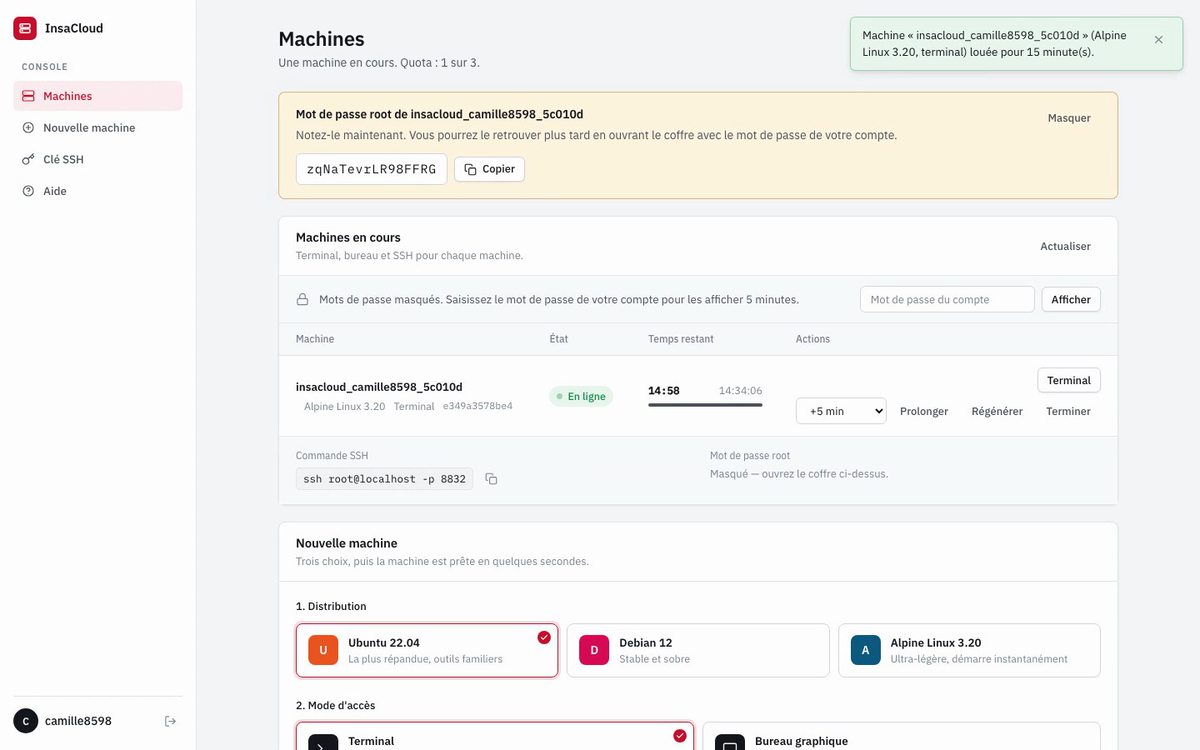
\includegraphics[width=\textwidth]{../docs/05-mot-de-passe-unique.png}
\end{minipage}\hfill
\begin{minipage}{0.48\textwidth}
  \centering
  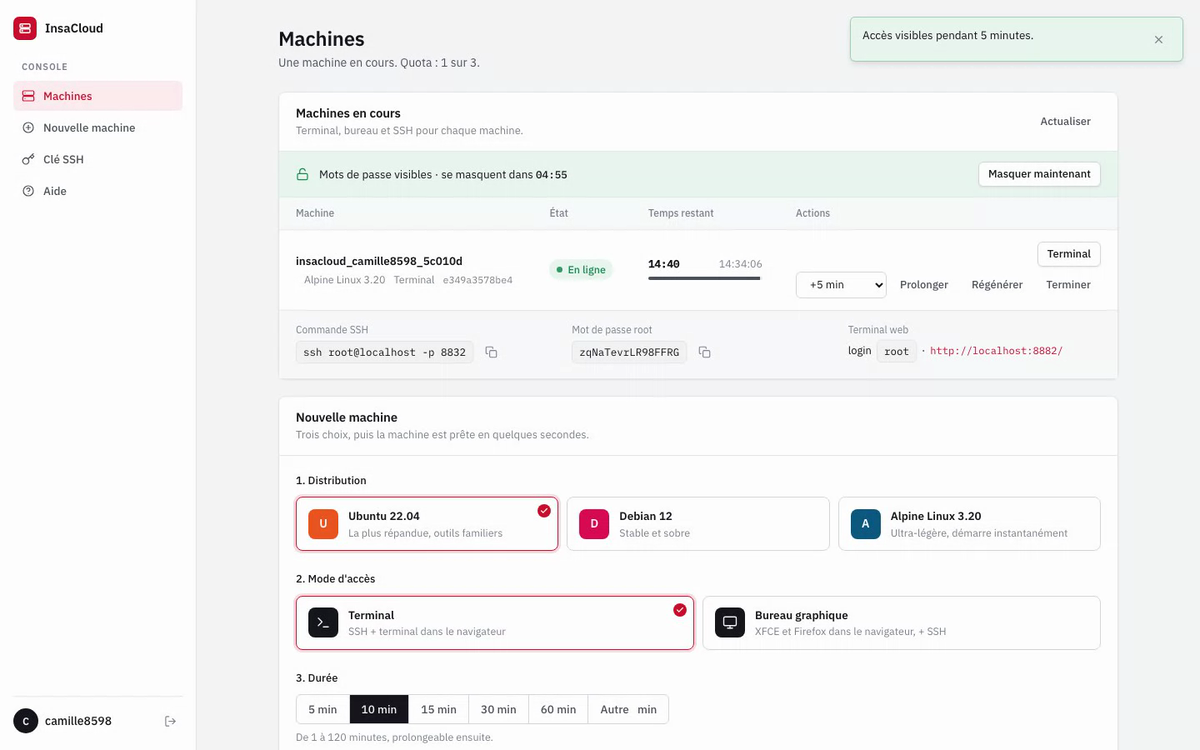
\includegraphics[width=\textwidth]{../docs/06-coffre-ouvert.png}
\end{minipage}
\caption{À gauche, l'affichage unique à la création. À droite, le coffre
rouvert après re-authentification : les accès redeviennent visibles cinq
minutes.}
\end{figure}

\begin{lstlisting}[language=Python,caption={\fichier{2\_webapp/app.py} --- plus rien de secret dans le cookie}]
def reveal_secret(instance_id: int, rotated: bool = False) -> None:
    # On ne depose que l'IDENTIFIANT de la machine dans la session. Le secret
    # lui-meme est relu en base, dechiffre, au moment de l'affichage.
    session["reveal"] = {"instance": int(instance_id), "rotated": bool(rotated)}

def secret_a_reveler():
    marqueur = session.pop("reveal", None)
    if not marqueur or g.user is None:
        return None
    # Le proprietaire est verifie dans la requete : l'identifiant d'une machine
    # d'autrui ne donne rien, meme si la session etait forgee.
    instance = db.get_instance(marqueur.get("instance"), user_id=g.user["id"])
    if instance is None or instance["status"] != db.STATUS_RUNNING:
        return None
    secret = decrypt_secret(instance["root_password"])
\end{lstlisting}

\section{CSRF : empêcher un autre site d'agir en votre nom}

\begin{notion}{\emph{Cross-Site Request Forgery}}
Vous êtes connecté à notre plateforme. Vous visitez un site malveillant qui
contient un formulaire invisible pointant vers \cmd{/instances/3/stop}, soumis
automatiquement. Votre navigateur joint vos cookies : la requête est
authentifiée, et votre machine s'arrête.

La parade : un jeton imprévisible, déposé dans la session et recopié dans
chaque formulaire. Le site malveillant ne peut pas le deviner --- il ne peut
pas lire votre session.
\end{notion}

\begin{piege}{Exempter les requêtes JSON, mais pourquoi ?}
L'API doit pouvoir être appelée par \cmd{curl}, qui n'a pas de jeton. Notre
exemption porte sur \cmd{Content-Type: application/json}, et elle est sûre pour
deux raisons :
\begin{itemize}
\item un formulaire HTML ne peut \emph{pas} émettre ce type de contenu --- il
  est limité à trois types, dont aucun n'est JSON ;
\item une requête \cmd{fetch} qui le fait depuis un autre site déclenche une
  vérification \emph{preflight} CORS, que le serveur refuse.
\end{itemize}
Le raisonnement compte autant que la règle : exempter sans comprendre ouvrirait
exactement le trou qu'on cherche à boucher.
\end{piege}

\begin{figure}[htbp]
\centering
\begin{minipage}{0.48\textwidth}
  \centering
  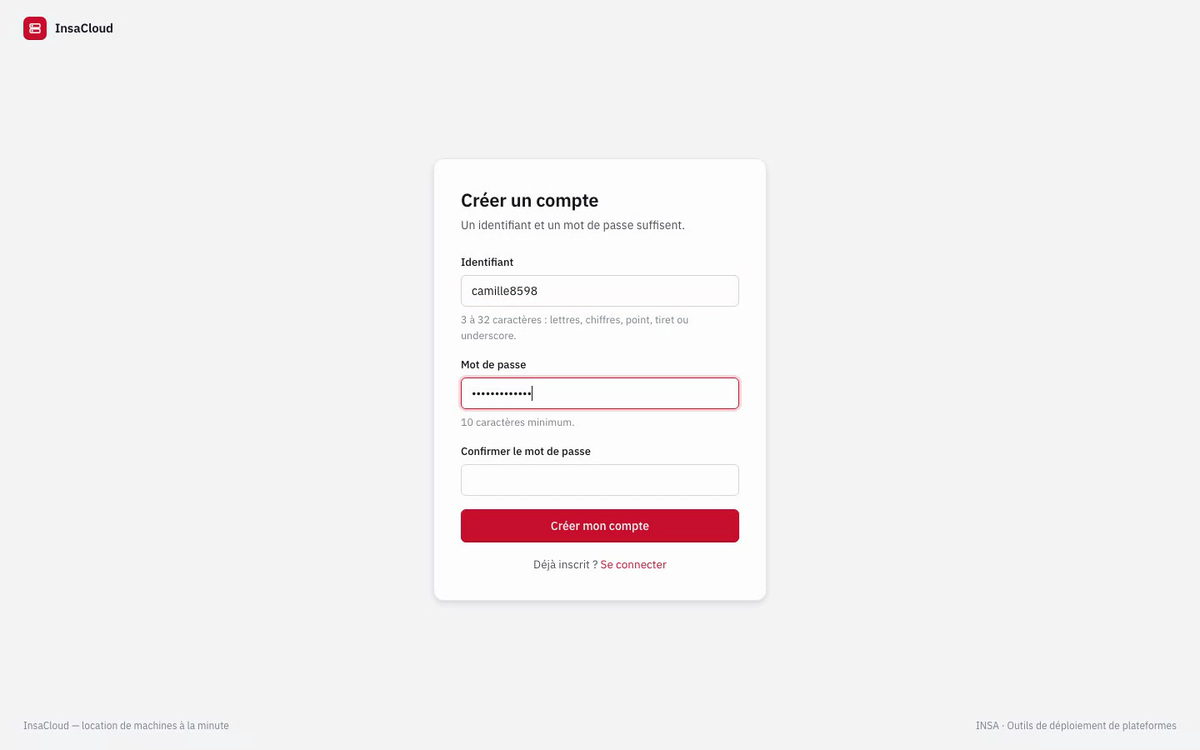
\includegraphics[width=\textwidth]{../docs/02-inscription.png}
\end{minipage}\hfill
\begin{minipage}{0.48\textwidth}
  \centering
  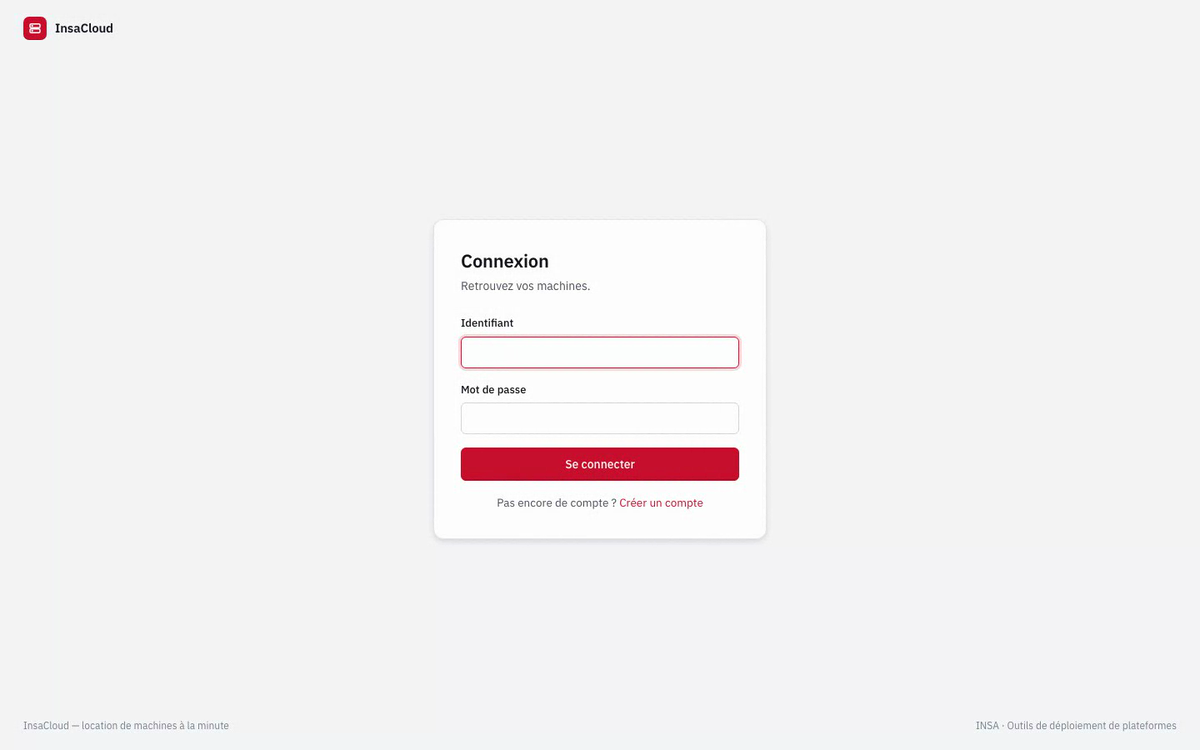
\includegraphics[width=\textwidth]{../docs/01-connexion.png}
\end{minipage}
\caption{Inscription et connexion. La politique de mot de passe est vérifiée
côté serveur : un contrôle fait uniquement dans le navigateur se contourne en
désactivant JavaScript.}
\end{figure}

\section{Empreinte et chiffrement, à ne pas confondre}

\begin{notion}{Deux besoins, deux mécanismes}
Le mot de passe d'un \emph{compte} est \textbf{haché} (\cmd{pbkdf2:sha256}) :
l'opération est à sens unique, on ne peut pas le retrouver, seulement vérifier
qu'un essai donne la même empreinte.

Le mot de passe \emph{root d'une machine louée} est \textbf{chiffré} : il doit
pouvoir être réaffiché, donc l'opération doit être réversible.

Hacher le second le rendrait inutilisable ; chiffrer le premier serait une
faute.
\end{notion}

Cinq échecs de connexion verrouillent temporairement le compte. Les tentatives
sont enregistrées avec l'adresse IP, dans une table indexée.

\section{Les en-têtes et la politique de contenu}

\begin{center}
\small
\begin{tabularx}{\textwidth}{@{}lX@{}}
\toprule
\textbf{En-tête} & \textbf{Effet} \\
\midrule
\cmd{Strict-Transport-Security} & le navigateur refuse ensuite le HTTP en clair \\
\cmd{X-Content-Type-Options} & interdit de deviner le type d'un fichier \\
\cmd{X-Frame-Options} & empêche l'inclusion du site dans un cadre \\
\cmd{Content-Security-Policy} & \cmd{default-src 'self'} : aucune ressource externe \\
\bottomrule
\end{tabularx}
\end{center}

\begin{retenir}
Une CSP stricte a un coût : plus de CDN, plus de script en ligne. Tailwind est
donc précompilé et les polices sont hébergées localement. C'est plus de travail
au départ, et cela supprime d'un coup toute une famille d'attaques par
injection de script.
\end{retenir}

\chapter{La haute disponibilité}
\label{chap:ha}

\section{Le scénario exact du cahier des charges}

L'énoncé décrit un test précis : éteindre un worker et vérifier que l'instance
repart ailleurs. Voici ce qui se passe, mesuré sur un cluster réel.

\begin{center}
\small
\begin{tabularx}{\textwidth}{@{}lX@{}}
\toprule
\textbf{Instant} & \textbf{Événement} \\
\midrule
T\,+\,0 s & \cmd{vagrant halt worker1} : l'agent cesse de battre \\
T\,+\,90 s & le Faucheur déclare \cmd{worker1} \cmd{OFFLINE} \\
T\,+\,90 s & la machine est recréée sur \cmd{worker2}, \cmd{migrations} passe à 1 \\
T\,+\,100 s & l'utilisateur voit un nouveau port et un nouveau mot de passe \\
plus tard & \cmd{worker1} redémarre, son agent se réinscrit en moins de 10 s \\
\bottomrule
\end{tabularx}
\end{center}

\begin{lstlisting}[language=Python,caption={\fichier{2\_webapp/services.py} --- la reprise}]
def recreer_ailleurs(instance: dict) -> Resultat:
    """
    Recree une instance sur un autre worker apres la panne du sien.

    Le conteneur est reconstruit a partir de la meme image, avec un mot de passe
    neuf — l'ancien vivait dans un conteneur devenu inaccessible. La location
    n'est pas touchee : l'utilisateur conserve la duree qu'il a payee.
    """
    ancien_noeud = instance["worker"]
    candidat = db.select_available_worker()
    if candidat is None or candidat["hostname"] == ancien_noeud:
        return Resultat.echec("Aucun worker de repli disponible.", code=503)
    ...
    db.move_instance(instance["id"], ports["container_id"], nouveau_noeud,
                     ports["port"], ports["term_port"], ports["gui_port"])
    db.set_instance_password(instance["id"], encrypt_secret(mot_de_passe))
\end{lstlisting}

Noter ce que ce code \emph{ne} fait pas : il ne touche pas à la table
\texttt{rentals}. C'est tout l'intérêt de la séparation du
chapitre~\ref{chap:modele}.

\section{Le compteur de migrations}

La colonne \cmd{migrations} de la table \texttt{instances} s'incrémente à
chaque reprise. Ce n'est pas décoratif : c'est la preuve observable qu'une
reprise a eu lieu, et c'est ce que vérifie le test d'intégration.

\begin{retenir}
Quand une fonctionnalité est difficile à observer, ajoutez-lui un compteur.
Sans \cmd{migrations}, il faudrait lire les journaux pour savoir si la reprise
a fonctionné --- et un test ne peut pas raisonnablement lire des journaux.
\end{retenir}

\chapter{Sauvegarder le travail avant destruction}
\label{chap:archives}

\section{Le besoin}

Détruire une machine détruit sa couche inscriptible. Un utilisateur qui a
travaillé trente minutes perd tout. Ce n'est demandé nulle part dans le cahier
des charges --- c'est un ajout, proposé par un contributeur extérieur et
intégré après correction.

\section{Le principe : un flux, pas un fichier temporaire}

\begin{lstlisting}[language=bash]
docker exec <conteneur> tar czf - -C / root home
\end{lstlisting}

Le tiret à la place du nom de fichier demande à \cmd{tar} d'écrire sur la
sortie standard. Python lit ce flux et l'écrit sur le disque du contrôleur. Pour
un worker distant, le transport SSH du client Docker fait passer le flux : rien
de plus n'est exposé sur le réseau, et rien n'est écrit dans le conteneur.

\begin{lstlisting}[language=Python,caption={\fichier{2\_webapp/archives.py} --- lire le flux sous contrainte}]
    # O_EXCL : on ne reecrit jamais un fichier existant. Mode 0600 des la
    # creation : l'archive peut contenir des cles ou des mots de passe.
    fd = os.open(destination, os.O_WRONLY | os.O_CREAT | os.O_EXCL, 0o600)
    with os.fdopen(fd, "wb") as sortie, subprocess.Popen(
            commande, stdout=subprocess.PIPE, stderr=subprocess.DEVNULL) as processus:

        def _delai():
            delai_depasse.set()
            processus.kill()

        minuteur = threading.Timer(ARCHIVE_TIMEOUT, _delai)
        minuteur.start()
        try:
            while bloc := processus.stdout.read(TAILLE_BLOC):
                taille += len(bloc)
                if taille > ARCHIVE_MAX_BYTES:
                    processus.kill()
                    return {"status": STATUS_TOO_LARGE}
                sortie.write(bloc)
                empreinte.update(bloc)
        finally:
            minuteur.cancel()
\end{lstlisting}

\begin{notion}{Pourquoi un minuteur et pas un test dans la boucle}
On pourrait vérifier le temps écoulé à chaque tour de boucle. Cela ne
marcherait pas : \cmd{read()} \emph{bloque} tant que Docker --- ou la connexion
SSH --- n'envoie rien. Si le nœud se fige, la boucle ne tourne plus du tout et
aucun test n'est évalué.

Un fil séparé qui tue le processus au bout du délai est la seule façon de
garantir la sortie.
\end{notion}

\section{La règle qui prime sur tout}

\begin{lstlisting}[language=Python,caption={\fichier{2\_webapp/archives.py} --- l'invariant du module}]
"""
Regle de conception : `archiver_conteneur` ne leve JAMAIS d'exception. Un
echec d'archivage (noeud injoignable, archive trop lourde, disque plein) doit
etre signale a l'appelant, pas l'empecher de detruire la machine : sinon une
machine expiree resterait en vie indefiniment.
"""
\end{lstlisting}

\begin{retenir}
Une fonctionnalité secondaire ne doit jamais pouvoir bloquer une fonctionnalité
essentielle. Ici, sauvegarder est un service rendu ; détruire à l'échéance est
une obligation. Si l'un doit céder, ce n'est pas le second.
\end{retenir}

\section{Retenter sans boucler}

La première version ne retentait jamais un archivage raté : une simple coupure
SSH condamnait les fichiers. Mais retenter à chaque cycle du Faucheur serait
pire : sur un nœud durablement muet, chaque passage attendrait le délai maximal
de 45 secondes, toutes les 10 secondes.

\begin{lstlisting}[language=Python,caption={\fichier{2\_webapp/database.py} --- le compromis}]
def archivage_deja_fait(instance_id: int, delai_avant_reprise: int = 600) -> bool:
    """
    Une archive reussie n'est jamais refaite : la destruction peut etre
    retentee pendant plusieurs cycles du Faucheur, le travail n'est copie
    qu'une fois.

    Un echec, en revanche, vient parfois d'un incident passager — un noeud
    brievement injoignable. On retente alors, mais pas a chaque cycle.
    """
\end{lstlisting}

\begin{notion}{Le téléchargement, et ses trois protections}
Une archive contient les fichiers privés d'un utilisateur. La route de
téléchargement les protège de trois façons :
\begin{enumerate}
\item le propriétaire est vérifié \emph{dans la requête SQL} : l'archive d'un
  autre compte répond 404, exactement comme une archive inexistante --- cela ne
  révèle rien sur les comptes voisins ;
\item \cmd{send\_from\_directory} joint le chemin au dossier des archives et
  refuse toute sortie (\cmd{../}), même si la base était altérée ;
\item la réponse est un téléchargement (\cmd{attachment}), jamais affichée
  dans la page.
\end{enumerate}
\end{notion}

\part{Le déploiement}
\label{part:deploiement}

\chapter{Monter le parc avec Vagrant}

\section{Quatre machines décrites en un fichier}

\begin{lstlisting}[language=Ruby,caption={\fichier{Vagrantfile} --- le parc, paramétrable}]
# Trois workers, comme le demande le cahier des charges. Sur un poste modeste,
# WORKERS=2 (ou 1) reduit le parc sans toucher au fichier :
#   WORKERS=2 vagrant up
NB_WORKERS = (ENV["WORKERS"] || "3").to_i.clamp(1, 9)

MACHINES = {
  "controller" => { "ip" => "192.168.56.10", "memory" => 2048, "cpus" => 2 },
}
(1..NB_WORKERS).each do |n|
  MACHINES["worker#{n}"] = { "ip" => "192.168.56.#{10 + n}",
                             "memory" => 3072, "cpus" => 2 }
end
\end{lstlisting}

\begin{retenir}
Rendre le nombre de workers paramétrable coûte trois lignes et change tout
pour qui lit le projet : on peut le faire tourner sur un portable avec un
seul worker, ou monter à neuf pour une démonstration. Un fichier qui n'offre
qu'une seule taille finit toujours par être modifié à la main --- et donc
désynchronisé.
\end{retenir}

\section{Plusieurs providers, et pourquoi}

\begin{lstlisting}[language=Ruby]
node.vm.provider "vmware_desktop" do |v| ... end
node.vm.provider "parallels"      do |p| ... end
node.vm.provider "qemu"           do |q, override| ... end
node.vm.provider "virtualbox"     do |v| ... end
\end{lstlisting}

VirtualBox, le provider par défaut, ne fonctionne pas sur les Mac à puce
Apple. Déclarer plusieurs providers permet au même fichier de marcher sur une
machine Intel, un Mac ARM et un poste Windows.

\begin{piege}{QEMU ne gère pas les réseaux privés}
Chaque provider a ses limites. \cmd{vagrant-qemu} ne sait pas créer de réseau
privé : l'accès SSH est redirigé sur \cmd{localhost}. Le \cmd{Vagrantfile} le
détecte et ajuste la configuration. Sans cela, le déploiement réussirait et
rien ne serait joignable.
\end{piege}

\section{Les commandes du quotidien}

\begin{lstlisting}[language=bash]
vagrant up                  # cree et demarre tout le parc
vagrant up worker2          # une seule machine
vagrant status              # qui tourne
vagrant ssh controller      # entrer dans une machine
vagrant halt worker1        # eteindre (le test de panne du cahier des charges)
vagrant reload worker1      # redemarrer
vagrant destroy -f          # tout effacer, pour repartir de zero
\end{lstlisting}

\chapter{Configurer avec Ansible}
\label{chap:ansible}

\section{La partition : quatre plays, neuf rôles}

\begin{lstlisting}[language=yamlplus,caption={\fichier{3\_ansible/site.yml} --- la structure}]
- name: 1. Durcissement de tous les noeuds (UFW)
  hosts: insacloud
  become: true
  roles:
    - role: security_hardening

- name: 2. Controleur — compte de service et cle SSH de pilotage
  hosts: controllers
  roles:
    - role: controller_key

- name: 3. Workers — Docker, certificat, acces du controleur, images
  hosts: workers
  roles:
    - role: docker
    - role: tls_cert
    - role: worker
    - role: docker_images
    - role: worker_agent

- name: 4. Controleur — client Docker, certificat, nginx, application
  hosts: controllers
  roles:
    - role: docker
    - role: tls_cert
    - role: reverse_proxy
    - role: webapp
\end{lstlisting}

\begin{notion}{Pourquoi cet ordre}
L'ordre n'est pas arbitraire. Le contrôleur doit avoir sa clé SSH
\emph{avant} que les workers n'autorisent cette clé ; les workers doivent
avoir Docker \emph{avant} qu'on y construise les images ; nginx doit être
configuré \emph{avant} que l'application démarre derrière lui.

Un playbook est une suite de dépendances. Les écrire explicitement évite les
« ça marche une fois sur deux ».
\end{notion}

\begin{center}
\small
\begin{tabularx}{\textwidth}{@{}lX@{}}
\toprule
\textbf{Rôle} & \textbf{Ce qu'il fait} \\
\midrule
\cmd{security\_hardening} & pare-feu UFW, ports ouverts selon le groupe \\
\cmd{controller\_key} & compte de service et clé SSH de pilotage \\
\cmd{docker} & Docker Engine sur les workers, client seul sur le contrôleur \\
\cmd{tls\_cert} & certificat auto-signé propre à chaque nœud \\
\cmd{worker} & accès SSH restreint du contrôleur, appartenance au groupe docker \\
\cmd{docker\_images} & construction des images des machines louées \\
\cmd{worker\_agent} & l'agent d'inscription et de battement de cœur \\
\cmd{reverse\_proxy} & nginx HTTPS devant Gunicorn \\
\cmd{webapp} & Flask, Gunicorn, Faucheur, watchdog, secrets \\
\bottomrule
\end{tabularx}
\end{center}

\section{Un piège réel : la déduplication des rôles}

Ansible n'exécute un rôle qu'une fois par play. Sauf si on l'appelle avec des
\emph{paramètres différents} : il le considère alors comme deux rôles
distincts et l'exécute deux fois.

Le rôle \cmd{docker} était appelé directement par le play du contrôleur, et
tiré en dépendance par \cmd{docker\_images}. Avec un paramètre différent à
chaque appel, il s'exécutait deux fois --- installant puis désinstallant le
démon.

\begin{lstlisting}[language=yamlplus,caption={La correction : une variable de play, pas un paramètre de rôle}]
- name: 4. Controleur
  hosts: controllers
  vars:
    single_host: "{{ groups['workers'] | default([]) | length == 0 }}"
    # Defini ici (et non en parametre de role) : un role appele avec des
    # parametres differents n'est pas dedoublonne par Ansible, et `docker` est
    # aussi tire comme dependance par `docker_images`. Une variable de play
    # s'applique aux deux appels, qui sont donc fusionnes en une execution.
    docker_cli_only: "{{ not single_host }}"
  roles:
    - role: docker
    - role: docker_images
      when: single_host
\end{lstlisting}

\begin{retenir}
Quand un comportement d'outil vous surprend, vérifiez-le par l'expérience
plutôt que par la documentation. Nous avons prouvé celui-ci en instrumentant
le rôle pour qu'il journalise chaque exécution.
\end{retenir}

\section{Les secrets : Ansible Vault}

\begin{lstlisting}[language=bash]
# Creer ou editer un fichier chiffre
ansible-vault create group_vars/insacloud/vault.yml
ansible-vault edit   group_vars/insacloud/vault.yml

# Jouer le playbook en fournissant la phrase de passe
ansible-playbook site.yml --ask-vault-pass
\end{lstlisting}

Le fichier est chiffré en AES-256 et peut être versionné sans danger. Il
contient la clé de session Flask, la clé du coffre Fernet, le mot de passe
PostgreSQL et le jeton des agents.

\begin{piege}{Un secret déposé dans une unité systemd}
Mettre \cmd{Environment=INSACLOUD\_VAULT\_KEY=...} dans un fichier d'unité le
rend lisible par n'importe qui : les unités sont en lecture pour tous, et
\cmd{systemctl show} les affiche.

La bonne façon : un fichier séparé en \cmd{0600}, appartenant au compte de
service, référencé par \cmd{EnvironmentFile=}. Le secret n'est alors ni dans
l'unité, ni dans les journaux.
\end{piege}

\section{Prouver l'idempotence}

\begin{lstlisting}[language=bash]
ansible-playbook site.yml --ask-vault-pass        # premier passage
ansible-playbook site.yml --ask-vault-pass        # second passage
\end{lstlisting}

Le second passage doit afficher \cmd{changed=0} sur chaque nœud. C'est mesuré
sur les quatre machines après chaque modification du projet.

\begin{center}
\small
\begin{verbatim}
PLAY RECAP ****************************************************************
controller : ok=71  changed=0  unreachable=0  failed=0  skipped=9
worker1    : ok=43  changed=0  unreachable=0  failed=0  skipped=4
worker2    : ok=43  changed=0  unreachable=0  failed=0  skipped=4
worker3    : ok=43  changed=0  unreachable=0  failed=0  skipped=4
\end{verbatim}
\end{center}

\begin{piege}{\texttt{command} et \texttt{shell} ne sont jamais idempotents}
Les modules \cmd{ansible.builtin.command} et \cmd{shell} exécutent ce qu'on
leur donne, sans rien vérifier : ils sont donc \emph{toujours} signalés
\cmd{changed}. Si vous devez les employer, ajoutez \cmd{creates:},
\cmd{removes:} ou \cmd{changed\_when:} pour leur apprendre à se taire quand il
n'y a rien à faire.
\end{piege}

\section{L'inventaire dynamique}

L'inventaire statique liste les machines à la main. Un inventaire
\emph{dynamique} les découvre.

\begin{lstlisting}[language=bash]
./inventaire_vagrant.py --list      # interroge Vagrant, produit du JSON
ansible-playbook -i inventaire_vagrant.py site.yml
\end{lstlisting}

Le script interroge \cmd{vagrant status} et construit les groupes. Changer le
nombre de VM ne demande plus de toucher à l'inventaire, et le déploiement
devient indépendant du provider de virtualisation.

\chapter{Servir l'application}

\section{nginx devant Gunicorn}

\begin{lstlisting}[language=bash,caption={Le principe de la configuration nginx}]
server {
    listen 443 ssl http2;
    ssl_protocols TLSv1.3;

    add_header Strict-Transport-Security "max-age=63072000" always;
    add_header X-Content-Type-Options nosniff always;

    location /static/ {
        alias /opt/insacloud/static/;    # servi par nginx, pas par Python
        expires 7d;
    }

    location / {
        proxy_pass http://127.0.0.1:5000;
        proxy_set_header Host $host;
        proxy_set_header X-Forwarded-For   $proxy_add_x_forwarded_for;
        proxy_set_header X-Forwarded-Proto $scheme;
    }
}
\end{lstlisting}

\begin{notion}{\texttt{X-Forwarded-For} et \texttt{ProxyFix}}
Derrière un proxy, toutes les requêtes semblent venir de \cmd{127.0.0.1}.
L'adresse réelle du client est placée par nginx dans l'en-tête
\cmd{X-Forwarded-For}.

Côté Flask, le \emph{middleware} \cmd{ProxyFix} lit ces en-têtes et rétablit
la bonne adresse. Sans lui, notre verrouillage anti-force-brute compterait
toutes les tentatives comme venant de la même IP --- et bloquerait tout le
monde au cinquième échec de n'importe qui.
\end{notion}

\section{systemd : faire tourner les services}

\begin{lstlisting}[caption={Le principe d'une unité systemd}]
[Unit]
Description=InsaCloud - application web
After=network-online.target

[Service]
User=insacloud
WorkingDirectory=/opt/insacloud
EnvironmentFile=/etc/insacloud/insacloud.env     # secrets, en 0600
ExecStart=/opt/insacloud/.venv/bin/gunicorn --preload -w 4 -b 127.0.0.1:5000 app:app
Restart=always
RestartSec=3

[Install]
WantedBy=multi-user.target
\end{lstlisting}

\begin{center}
\small
\begin{tabularx}{\textwidth}{@{}lX@{}}
\toprule
\textbf{Directive} & \textbf{Effet} \\
\midrule
\cmd{User=} & le service ne tourne pas en root \\
\cmd{EnvironmentFile=} & les secrets viennent d'un fichier protégé, pas de l'unité \\
\cmd{Restart=always} & systemd relance le service s'il meurt \\
\cmd{After=network-online} & ne pas démarrer avant que le réseau soit prêt \\
\cmd{--preload} & Gunicorn importe l'application une fois, puis duplique \\
\bottomrule
\end{tabularx}
\end{center}

\section{Le watchdog}

Un \emph{timer} systemd vérifie chaque minute que nginx répond, que le site
renvoie bien du HTTPS, et que le Faucheur tourne. Il redémarre ce qui est
tombé et journalise les workers injoignables.

\begin{notion}{Timer plutôt que cron}
Un timer systemd s'intègre aux journaux (\cmd{journalctl -u ...}), connaît
l'état du service qu'il surveille, et ne démarre pas avant que ses
dépendances soient prêtes. Cron ne sait rien de tout cela.
\end{notion}

\chapter{La pile \texttt{docker compose}}

\section{Pourquoi une seconde façon de déployer}

Monter quatre VM demande du temps, de la mémoire et un hyperviseur. Pour
développer, démontrer, ou faire tourner les tests d'intégration en
intégration continue, on veut une pile en une commande.

\begin{lstlisting}[language=bash]
cp .env.example .env         # puis renseigner les secrets
docker compose up -d
\end{lstlisting}

\section{Un bloc partagé par deux services}

\begin{lstlisting}[language=yamlplus,caption={\fichier{docker-compose.yml} --- l'ancre YAML}]
x-application: &application
  build:
    context: ./2_webapp
  image: insacloud_web:latest
  restart: unless-stopped
  environment:
    INSACLOUD_ENV: production
    INSACLOUD_CLUSTER: ${INSACLOUD_CLUSTER:-compose}
    DATABASE_URL: "postgresql+psycopg://...:${POSTGRES_PASSWORD:?manquant}@db:5432/..."
    INSACLOUD_SECRET_KEY: ${INSACLOUD_SECRET_KEY:?definissez INSACLOUD_SECRET_KEY}
  depends_on:
    db:
      condition: service_healthy

services:
  web:
    <<: *application              # reprend tout le bloc ci-dessus
    ports: ["127.0.0.1:8088:5000"]
  faucheur:
    <<: *application
    command: ["python", "faucheur.py"]
\end{lstlisting}

\begin{notion}{Les ancres YAML}
\cmd{\&application} donne un nom à un bloc ; \cmd{<<: *application} le
recopie. L'application et le Faucheur partagent ainsi exactement la même
configuration --- il devient impossible qu'ils divergent sur une variable.
\end{notion}

\begin{notion}{\texttt{\$\{VAR:?message\}}}
Cette syntaxe refuse de démarrer si la variable n'est pas définie, en
affichant le message. La pile ne peut donc pas tourner avec un mot de passe
vide ou une clé par défaut : l'erreur arrive au démarrage, pas trois semaines
plus tard.
\end{notion}

\section{Le volume partagé, et pourquoi il ne s'invente pas}

\begin{lstlisting}[language=yamlplus]
  web:
    volumes:
      - /var/run/docker.sock:/var/run/docker.sock
      - archives_travail:/var/lib/insacloud/archives
  faucheur:
    volumes:
      - /var/run/docker.sock:/var/run/docker.sock
      - archives_travail:/var/lib/insacloud/archives

volumes:
  donnees_postgres:
  archives_travail:
\end{lstlisting}

\begin{piege}{Deux services, un seul dossier}
Le Faucheur \emph{écrit} l'archive ; l'application la \emph{sert} au
téléchargement. Si chacun avait son propre volume, l'utilisateur verrait dans
son tableau de bord une archive que le serveur ne trouverait pas.

Le même volume nommé doit donc être monté dans les deux services. C'est le
genre d'erreur qui ne se voit pas à la lecture du fichier, et qui saute aux
yeux au premier essai réel.
\end{piege}

\begin{piege}{La socket Docket donne les pleins pouvoirs}
Monter \cmd{/var/run/docker.sock} dans un conteneur lui donne un pouvoir
équivalent à root sur l'hôte : il peut créer un conteneur privilégié qui monte
le disque entier. C'est acceptable sur un poste de développement, jamais en
production --- où le contrôleur pilote des workers distants par SSH et n'a
plus besoin de cette ligne.
\end{piege}

\section{Les profils}

\begin{lstlisting}[language=bash]
docker compose up -d                        # la plateforme seule
docker compose --profile build build        # + construire les six images
docker compose --profile demo up -d         # + une machine de demonstration
\end{lstlisting}

Un service marqué d'un profil ne démarre que si on le demande. Cela permet de
décrire dans un seul fichier la pile minimale et tous ses compléments.

\part{La vérification}
\label{part:verification}

\chapter{Les tests}

\section{Tester Docker sans Docker}

Le problème est concret : les tests doivent tourner sur un agent d'intégration
qui n'a pas forcément Docker, et ils doivent être rapides. Lancer de vrais
conteneurs prendrait des minutes et échouerait au moindre réseau capricieux.

La solution : remplacer \cmd{run\_docker} par une fonction espion qui note ce
qu'on lui demande, sans rien exécuter.

\begin{lstlisting}[language=Python,caption={Le principe de l'espion}]
def test_la_commande_imposee_est_bien_celle_qui_part(monkeypatch):
    appels = []
    monkeypatch.setattr(docker_ops, "run_docker",
                        lambda *a, **k: appels.append(a) or "abc123def456")

    docker_ops.docker_run_container(port=8001, name="insacloud_test", ...)

    args = appels[0]
    assert "run" in args and "-d" in args
    assert "--restart=always" in args
    assert "-p" in args and "8001:22" in args
\end{lstlisting}

\begin{notion}{\emph{monkeypatch} et double de test}
\cmd{monkeypatch} est une fonctionnalité de pytest qui remplace un attribut le
temps d'un test, puis le restaure. On parle de \emph{double de test} : un
objet qui prend la place du vrai pour la durée de l'essai.

Ici, cela permet de vérifier que la commande imposée par l'énoncé
--- \cmd{docker run -d --restart=always -p <port>:22} --- est bien celle qui
part, sur une machine qui n'a pas Docker.
\end{notion}

\section{Partir d'une base vierge à chaque test}

\begin{lstlisting}[language=Python,caption={\fichier{2\_webapp/tests/conftest.py}}]
@pytest.fixture(autouse=True)
def base_vierge():
    """
    Chaque test part d'une base vide : aucun test n'herite de l'etat d'un autre.

    Le moteur SQLAlchemy est ferme avant d'effacer le fichier : sans cela, les
    connexions du pool continueraient de pointer sur l'ancien fichier efface.
    """
    db.engine.dispose()
    try:
        os.remove(db.DB_PATH)
    except FileNotFoundError:
        pass
    db.init_db()
    yield
\end{lstlisting}

\begin{piege}{Des tests qui dépendent de leur ordre}
Si un test laisse des données derrière lui, le suivant peut réussir pour la
mauvaise raison --- ou échouer quand on le lance seul. Le symptôme :
« ça passe en entier mais pas tout seul », ou l'inverse.

\cmd{autouse=True} applique la remise à zéro à \emph{tous} les tests, sans
qu'on ait à y penser.
\end{piege}

\section{Préparer l'environnement avant l'import}

\begin{lstlisting}[language=Python,caption={\fichier{2\_webapp/tests/conftest.py} --- l'ordre compte}]
# --- Environnement de test, fixe AVANT l'import de l'application -------------
_TMP = tempfile.mkdtemp(prefix="insacloud-tests-")
os.environ["INSACLOUD_DB"] = os.path.join(_TMP, "test.db")
os.environ["INSACLOUD_SECRET_KEY"] = "cle-de-session-de-test-uniquement"
os.environ["INSACLOUD_VAULT_KEY"] = Fernet.generate_key().decode()
os.environ["INSACLOUD_WORKERS"] = ""          # mode mono-hote

import pytest                                 # noqa: E402
import app as insacloud                       # noqa: E402
\end{lstlisting}

\begin{retenir}
L'application lit sa configuration \emph{au moment de l'import}. Si l'on
importait \cmd{app} avant de poser ces variables, les tests écriraient dans la
vraie base du poste de développement et utiliseraient les vraies clés. L'ordre
des lignes de ce fichier est donc une mesure de sécurité, pas un détail de
style.
\end{retenir}

\section{Ce que couvrent les 169 tests}

\begin{center}
\small
\begin{tabularx}{\textwidth}{@{}lrX@{}}
\toprule
\textbf{Fichier} & \textbf{Tests} & \textbf{Ce qu'il vérifie} \\
\midrule
\cmd{test\_securite.py} & 32 & CSRF, anti-force-brute, cloisonnement entre comptes, en-têtes, coffre \\
\cmd{test\_workers.py} & 37 & inscription, battement de cœur, états, ordonnanceur, reprise, libération du nom \\
\cmd{test\_docker.py} & 24 & la commande construite, le durcissement, les labels \\
\cmd{test\_faucheur.py} & 17 & expiration, réconciliation par nœud, nœud injoignable \\
\cmd{test\_contraintes.py} & 8 & index unique partiel, unicité, clés étrangères, idempotence, pool après fork \\
\cmd{test\_archives*.py} & 51 & archivage, purge, téléchargement, reprise après échec \\
\midrule
\textbf{Total} & \textbf{169} & en 20 secondes, sans Docker ni réseau \\
\bottomrule
\end{tabularx}
\end{center}

\section{Le test de cloisonnement, le plus important}

\begin{lstlisting}[language=Python,caption={Vérifier qu'un compte ne voit pas les machines d'un autre}]
def test_un_utilisateur_ne_voit_pas_la_machine_d_un_autre(client):
    # Alice loue une machine
    inscrire(client, "alice"); loue = louer(client)
    client.post("/logout")

    # Bob se connecte et tente d'y acceder par son identifiant
    inscrire(client, "bob")
    reponse = client.get(f"/instances/{loue['id']}")

    # 404, pas 403 : repondre « interdit » confirmerait que la machine existe
    assert reponse.status_code == 404
\end{lstlisting}

\begin{notion}{404 plutôt que 403}
Répondre « accès interdit » révèle que la ressource existe. En énumérant les
identifiants, un attaquant apprendrait combien de machines tournent et
lesquelles. Répondre « introuvable » ne distingue pas « n'existe pas » de
« ne vous appartient pas ».

C'est pourquoi le filtre sur le propriétaire est placé \emph{dans la requête
SQL} plutôt que dans un test après coup : il devient impossible d'oublier.
\end{notion}

\section{Les tests d'intégration : la vraie pile}

Les tests unitaires ne lancent rien. Un second niveau monte la pile complète et
la parcourt :

\begin{lstlisting}[language=bash]
./tests/integration.sh http://127.0.0.1:8088
\end{lstlisting}

\begin{center}
\small
\begin{tabularx}{\textwidth}{@{}lX@{}}
\toprule
\textbf{Scénario} & \textbf{Ce qu'il prouve} \\
\midrule
1. Infrastructure & les nœuds sont là et se parlent \\
2. Configuration & Ansible a fait son travail \\
3. Application & inscription, connexion, tableau de bord \\
4. Location & louer une machine et s'y connecter en SSH \\
5. Expiration & une location échue est réellement détruite \\
6. Panne & un nœud tombe, la machine repart ailleurs \\
\bottomrule
\end{tabularx}
\end{center}

\begin{piege}{Le port est publié avant que le service écoute}
Docker publie le port dès la création du conteneur, mais \cmd{sshd} met une
seconde ou deux à démarrer. Un test qui se connecte immédiatement échoue de
façon intermittente.

La correction n'est pas d'attendre « assez longtemps » --- une durée fixe est
toujours trop courte un jour et trop longue tous les autres --- mais de
réessayer jusqu'à ce que le service réponde, avec une limite.
\end{piege}

\chapter{La chaîne d'intégration}
\label{chap:ci}

\section{Onze travaux}

\begin{figure}[htbp]
\centering
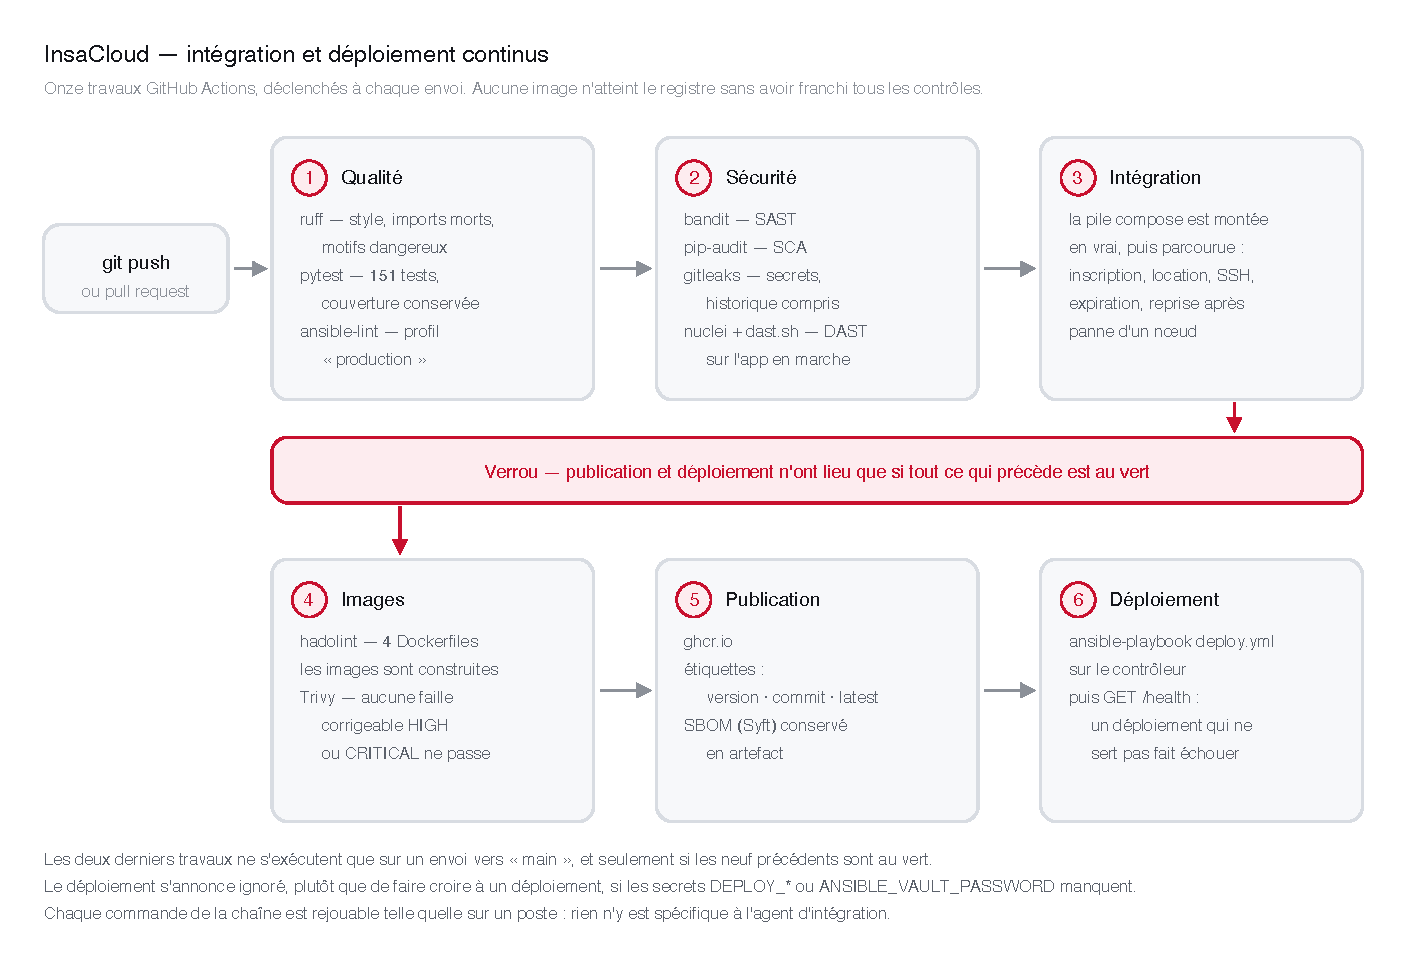
\includegraphics[width=\textwidth]{figures/chaine-ci-cd.pdf}
\caption{Les onze travaux et le verrou qui protège le registre.}
\end{figure}

\begin{center}
\small
\begin{tabularx}{\textwidth}{@{}llX@{}}
\toprule
\textbf{Travail} & \textbf{Outil} & \textbf{Ce qu'il attrape} \\
\midrule
Lint Python & \cmd{ruff} & imports morts, noms inconnus, motifs douteux \\
Tests & \cmd{pytest} & 169 cas, couverture conservée en artefact \\
SAST & \cmd{bandit} & injection, secrets en dur, appels système risqués \\
SCA & \cmd{pip-audit} & CVE des dépendances épinglées \\
Secrets & \cmd{gitleaks} & clés commises, y compris dans l'historique \\
DAST & \cmd{dast.sh} + \cmd{nuclei} & l'application en fonctionnement \\
Lint Ansible & \cmd{ansible-lint} & rôles, profil \cmd{production} \\
Images & \cmd{hadolint} + \cmd{Trivy} & 4 Dockerfiles, CVE des images \\
Intégration & \cmd{docker compose} & la pile démarre et une machine se loue \\
Publication & \cmd{Syft} + \cmd{ghcr.io} & SBOM conservé, images étiquetées \\
Déploiement & \cmd{ansible-playbook} & met à jour l'hôte puis interroge \cmd{/health} \\
\bottomrule
\end{tabularx}
\end{center}

\section{Le verrou}

Les deux derniers travaux ne s'exécutent que sur un envoi vers \cmd{main}, et
seulement si les neuf précédents sont au vert :

\begin{lstlisting}[language=yamlplus]
  publier-images:
    needs: [lint-python, tests-python, sast-python, sca-dependances, secrets,
            dast, lint-ansible, images-docker, integration]
    if: github.event_name == 'push' && github.ref == 'refs/heads/main'
\end{lstlisting}

\begin{retenir}
Sans \cmd{needs:}, GitHub Actions lance tous les travaux en parallèle --- et
publierait l'image pendant que les tests échouent. La dépendance explicite
est ce qui transforme une liste de contrôles en une véritable barrière.
\end{retenir}

\section{Trois incidents instructifs}

\paragraph{Nos images refusées par notre propre scan.} Le travail
\cmd{images-docker} refuse toute faille corrigeable de niveau HIGH ou
CRITICAL. Notre image utilisait \cmd{docker:28-cli}, qui traînait 163 failles
corrigeables liées à sa version de Go, plus des CVE OpenSSL héritées de la
base Debian.

La correction a tenu en deux gestes : passer à \cmd{docker:29-cli} (2 failles
au lieu de 163) et ajouter un \cmd{apt-get upgrade} pour OpenSSL. Le verrou
utilise par ailleurs \cmd{--ignore-unfixed} : refuser une faille sans correctif
disponible ne protégerait de rien et bloquerait tout.

\paragraph{Une dépendance qui n'existe pas pour la cible.} Le projet épinglait
SQLAlchemy 2.1.1, disponible sur notre poste. La cible de déploiement est
Ubuntu 22.04, qui fournit Python 3.10 --- pour lequel cette version n'a jamais
été publiée. Les tests passaient, le déploiement échouait.

\paragraph{Deux guillemets déséquilibrées.} Une erreur de syntaxe shell dans un
bloc \cmd{run:} ne se voit qu'au moment où l'étape s'exécute, parfois après dix
minutes de chaîne. Trois exécutions ont échoué ainsi. Nous avons ajouté un
contrôle qui extrait chaque bloc \cmd{run:}, neutralise les expressions
\cmd{\$\{\{ \}\}} et passe le tout à \cmd{bash -n} :

\begin{lstlisting}[language=yamlplus,caption={\fichier{.github/workflows/ci.yml} --- la chaîne vérifie sa propre syntaxe}]
      - name: Verifier la syntaxe shell de la chaine elle-meme
        run: |
          pip install --quiet pyyaml
          python3 .github/verifier-workflow.py
\end{lstlisting}

\begin{retenir}
Chaque fois qu'un défaut vous a coûté du temps, demandez-vous quel contrôle
automatique l'aurait attrapé --- puis ajoutez-le. Une chaîne d'intégration
n'est pas écrite d'un coup : elle se construit par sédimentation, un incident
après l'autre.
\end{retenir}

\section{Empêcher la documentation de vieillir}

Les schémas du dépôt sont engendrés par des scripts Python ; la chaîne les
régénère et refuse la moindre différence :

\begin{lstlisting}[language=yamlplus]
      - name: Verifier que les schemas du README sont a jour
        run: |
          python3 docs/schemas/tout.py
          git diff --exit-code -- docs/*.svg
\end{lstlisting}

\begin{piege}{Du texte à jour, des images périmées}
Ce garde-fou vient d'une erreur réelle. Le README avait été mis à jour ---
texte, chiffres, descriptions d'images --- mais les schémas SVG, eux,
montraient encore deux workers alors que le projet en comptait trois.

La moitié du contenu d'un README est visuelle. La traiter comme du texte, c'est
garantir qu'elle finira fausse.
\end{piege}

\chapter{Ce qu'on a trouvé en faisant tourner}

Les défauts qui suivent n'ont pas été trouvés en relisant le code, mais en le
faisant fonctionner : en déployant sur un cluster, en lançant la pile, en
lisant les journaux.

\begin{center}
\small
\begin{tabularx}{\textwidth}{@{}XX@{}}
\toprule
\textbf{Défaut} & \textbf{Garde-fou ajouté} \\
\midrule
Le Faucheur détruisait sa propre plateforme : il reconnaissait les machines
à leur préfixe de nom &
Identité par étiquette Docker, plus jamais par nom ; un test le vérifie \\
\addlinespace
Deux déploiements sur un même démon se supprimaient mutuellement leurs
conteneurs &
Un second label délimite le déploiement \\
\addlinespace
Le mot de passe de la base journalisé en clair au démarrage du Faucheur &
Toute URL passe par une fonction de masquage \\
\addlinespace
Une dépendance épinglée inexistante pour le Python de la cible &
La chaîne installe exactement \cmd{requirements.txt} sur la cible réelle \\
\addlinespace
Des distributions proposées sans image construite &
Le catalogue interroge Docker avant d'afficher un choix \\
\addlinespace
Course au démarrage entre les quatre processus Gunicorn &
Création tolérante à la concurrence, et \cmd{--preload} \\
\addlinespace
Images refusées par notre propre scan Trivy &
Base plus récente, \cmd{apt-get upgrade}, \cmd{--ignore-unfixed} \\
\addlinespace
Deux guillemets déséquilibrées dans la chaîne elle-même &
Un contrôle de syntaxe shell de tous les blocs \cmd{run:} \\
\addlinespace
Le mot de passe root lisible dans le cookie de session &
Seul l'identifiant transite ; le secret est relu chiffré en base \\
\addlinespace
Les schémas du README figés sur une ancienne architecture &
La chaîne régénère les SVG et refuse toute différence \\
\bottomrule
\end{tabularx}
\end{center}

\begin{retenir}
Dix défauts, dix garde-fous. C'est la différence entre « on a corrigé » et
« cela ne peut plus revenir ». Corriger sans ajouter de contrôle, c'est
accepter de recommencer.
\end{retenir}

\section{Ce qui a été vérifié sur un cluster réel}

\begin{itemize}
\item \textbf{Déploiement complet} : \cmd{failed=0} sur les quatre nœuds.
\item \textbf{Idempotence} : second passage à \cmd{changed=0} sur les quatre.
\item \textbf{Inscription spontanée} : les trois agents se sont enregistrés
  seuls, aucune adresse de worker n'étant écrite côté contrôleur.
\item \textbf{Parcours utilisateur} : inscription, location, accès ; le
  conteneur est bien créé sur le nœud le moins chargé.
\item \textbf{Durcissement effectif} : \cmd{docker inspect} confirme
  \cmd{restart=always}, les limites mémoire, \cmd{pids-limit},
  \cmd{cap-drop ALL} et \cmd{no-new-privileges}.
\item \textbf{Conservation de l'état} : après redémarrage du démon Docker
  \emph{puis} du nœud entier, la machine et le travail de l'utilisateur sont
  intacts.
\item \textbf{Faucheur} : une location d'une minute détruite 49 secondes après
  son expiration.
\item \textbf{Reprise sur panne} : le scénario de l'énoncé joué tel quel.
\item \textbf{Analyse dynamique} : 18 contrôles sur l'application en
  fonctionnement, tous réussis.
\end{itemize}

\part{Annexes}

\chapter{Refaire le projet depuis zéro}

Voici l'ordre dans lequel aborder un projet de ce type. Chaque étape produit
quelque chose qui marche : c'est ce qui permet de ne jamais se retrouver avec
mille lignes dont rien ne fonctionne.

\begin{enumerate}
\item \textbf{Un conteneur SSH à la main.} Écrivez un Dockerfile qui installe
  \cmd{openssh-server}, lancez-le avec \cmd{-p 2222:22}, connectez-vous.
  Objectif : comprendre la publication de port.
\item \textbf{Plusieurs services dedans.} Ajoutez \cmd{supervisord} et un
  terminal web. Objectif : comprendre PID 1.
\item \textbf{Une page Flask qui lance ce conteneur.} Un bouton, un
  \cmd{subprocess}, un message. Pas de base, pas de comptes.
\item \textbf{Une base.} Enregistrez ce que vous créez. Séparez dès maintenant
  la machine de la location : ce choix est difficile à rattraper après coup.
\item \textbf{Des comptes.} Inscription, connexion, et surtout le cloisonnement
  --- un utilisateur ne voit que ses machines.
\item \textbf{L'expiration.} Un script séparé qui boucle et détruit. Testez-le
  avec des locations d'une minute.
\item \textbf{Les tests.} Maintenant, pas plus tard : vous avez assez de code
  pour que les régressions commencent.
\item \textbf{Un second nœud.} C'est là que tout change : SSH, ordonnanceur,
  agent. Faites-le avant d'avoir trop de code supposant un hôte unique.
\item \textbf{Ansible.} Automatisez ce que vous faites à la main depuis le
  début. Visez \cmd{changed=0} au second passage dès le premier jour.
\item \textbf{La chaîne d'intégration.} Commencez par lint et tests, ajoutez
  le reste progressivement.
\item \textbf{La haute disponibilité.} Éteignez un nœud et regardez ce qui se
  passe. Corrigez. Recommencez.
\end{enumerate}

\begin{retenir}
L'ordre compte plus qu'on ne croit. Ajouter le multi-nœuds à la fin oblige à
réécrire tout le code qui appelait \cmd{docker} sans se demander « sur quelle
machine ? ». Ajouter les tests à la fin revient à ne pas les ajouter.
\end{retenir}

\chapter{Commandes utiles}

\section{Le projet}

\begin{lstlisting}[language=bash]
# --- Pile complete en local --------------------------------------------------
cp .env.example .env                     # puis renseigner les secrets
docker compose up -d
docker compose --profile build build     # construire les six images
docker compose logs -f web
docker compose down -v                   # tout effacer, volumes compris

# --- Developpement -----------------------------------------------------------
cd 2_webapp
python3 -m venv .venv && .venv/bin/pip install -r requirements-dev.txt
.venv/bin/python app.py                  # serveur de developpement

# --- Controles, les memes que la chaine --------------------------------------
pytest                                   # 169 tests
ruff check .
bandit -c pyproject.toml -r .
pip-audit -r requirements.txt
alembic check
./tests/dast.sh http://127.0.0.1:5000
./tests/integration.sh http://127.0.0.1:8088

# --- Cluster -----------------------------------------------------------------
vagrant up
cd 3_ansible && ansible-playbook site.yml --ask-vault-pass
ansible-playbook site.yml --ask-vault-pass    # doit donner changed=0
vagrant halt worker1                     # le test de panne
\end{lstlisting}

\section{Diagnostiquer}

\begin{lstlisting}[language=bash]
# Que fait reellement un conteneur ?
docker inspect <conteneur> | jq '.[0].HostConfig | {Memory, NanoCpus, CapDrop, PidsLimit}'

# Pourquoi ne demarre-t-il pas ?
docker logs <conteneur>

# Quelles machines la plateforme reconnait-elle comme siennes ?
docker ps -a --filter "label=insacloud.role=rented-machine"

# Les services sur le controleur
systemctl status insacloud insacloud-faucheur nginx
journalctl -u insacloud-faucheur -f

# L'etat du parc, vu de l'exterieur
curl -s http://127.0.0.1:8088/health | jq
curl -s -H 'Accept: application/json' http://127.0.0.1:8088/workers | jq
\end{lstlisting}

\chapter{Erreurs fréquentes}

\begin{center}
\small
\begin{tabularx}{\textwidth}{@{}XX@{}}
\toprule
\textbf{Symptôme} & \textbf{Cause probable} \\
\midrule
\cmd{exec format error} ou \cmd{no such file or directory} sur un script qui
existe pourtant &
Le script a des fins de ligne Windows (CRLF). Le \cmd{\textbackslash r} fait
partie du nom de l'interpréteur dans le shebang. Corriger avec un
\cmd{.gitattributes} : \cmd{* text=auto eol=lf} \\
\addlinespace
\cmd{port is already allocated} &
Un conteneur précédent n'a pas été nettoyé, ou deux requêtes ont choisi le même
port. L'index unique partiel règle le second cas \\
\addlinespace
\cmd{table users already exists} au démarrage &
Plusieurs processus Gunicorn créent le schéma en même temps. Utiliser
\cmd{--preload} et tolérer l'erreur \\
\addlinespace
Le conteneur démarre puis s'arrête aussitôt &
Son processus principal s'est terminé. Un conteneur vit tant que son PID 1 vit \\
\addlinespace
\cmd{permission denied} sur \cmd{/var/run/docker.sock} &
Le compte n'est pas dans le groupe \cmd{docker}. En conteneur, utiliser
\cmd{group\_add} avec le GID de l'hôte \\
\addlinespace
Ansible affiche \cmd{changed} à chaque passage &
Un module \cmd{command} ou \cmd{shell} sans \cmd{creates:} ni
\cmd{changed\_when:} \\
\addlinespace
Le site répond en HTTP mais pas en HTTPS &
Certificat absent ou illisible par nginx, ou port 443 fermé par UFW \\
\addlinespace
Tout le monde est bloqué par l'anti-force-brute &
\cmd{ProxyFix} n'est pas actif : toutes les requêtes semblent venir du proxy \\
\addlinespace
Les tests passent ensemble mais échouent seuls (ou l'inverse) &
Un test laisse des données derrière lui. Remettre la base à zéro avec une
fixture \cmd{autouse} \\
\addlinespace
La connexion SSH échoue juste après la location &
Docker publie le port avant que \cmd{sshd} écoute. Réessayer avec une limite,
plutôt qu'attendre une durée fixe \\
\bottomrule
\end{tabularx}
\end{center}

\chapter{Conformité au cahier des charges}

\begin{center}
\small
\begin{tabularx}{\textwidth}{@{}llX@{}}
\toprule
\textbf{\#} & \textbf{Fonctionnalité} & \textbf{Réalisation} \\
\midrule
1 & Préparation et environnement & dépôt Git, environnement virtuel, dépendances épinglées \\
2 & API Web Flask & modules séparés, comptes, sessions, tableau de bord \\
3 & Base de données & 7 tables en SQLAlchemy, migrations Alembic, index métier \\
4 & Conteneurisation Docker & 4 Dockerfiles, 6 images, durcissement complet \\
5 & Infrastructure Vagrant & 4 VM, réseau privé, 4 providers \\
6 & Automatisation Ansible & 9 rôles, 4 playbooks, Vault, idempotence mesurée \\
7 & Worker Agent & inscription spontanée, battement de cœur, 3 états \\
8 & Ordonnanceur & nœud joignable le moins chargé, départage déterministe \\
9 & Service de location & durée 1--120 min, prolongation, arrêt \\
10 & Déploiement des instances & la commande imposée, par \cmd{subprocess} \\
11 & Accès SSH & par mot de passe ou par clé, plus terminal web et bureau \\
12 & Expiration & le Faucheur, toutes les 10 s, avec réconciliation \\
13 & Haute disponibilité & 3 niveaux, scénario de l'énoncé vérifié \\
14 & Sécurité DevSecOps & SAST, SCA, secrets, DAST, scan d'image, SBOM \\
15 & CI/CD & 11 travaux, publication conditionnelle, déploiement vérifié \\
16 & Tests d'intégration & 169 tests unitaires + 6 scénarios de bout en bout \\
17 & Documentation & README, guide d'API, schéma de base, ce guide \\
\bottomrule
\end{tabularx}
\end{center}

\section*{Au-delà de l'énoncé}

\begin{itemize}
\item Architecture distribuée à trois workers, alors qu'un seul hôte suffisait.
\item Terminal web et bureau graphique complet dans le navigateur, en plus du
  SSH demandé.
\item Coffre à secrets : mot de passe root chiffré, réaffichable après
  re-authentification.
\item Watchdog systemd d'auto-réparation du service.
\item Inventaire dynamique interrogeant Vagrant.
\item Sauvegarde du travail avant destruction, téléchargeable sept jours.
\item Schémas engendrés depuis leur description, et contrôlés par la chaîne.
\end{itemize}

\chapter{Glossaire}

\begin{description}
\item[Agent] petit programme tournant sur chaque worker, qui l'inscrit auprès
  du contrôleur et signale régulièrement sa présence.
\item[Alembic] outil de migration de schéma pour SQLAlchemy.
\item[Ansible] outil de configuration qui applique un état décrit en YAML, par
  SSH, de façon idempotente.
\item[Capacité (\emph{capability})] fraction des pouvoirs de root, attribuable
  indépendamment des autres.
\item[cgroup] mécanisme du noyau Linux limitant les ressources qu'un groupe de
  processus peut consommer.
\item[CSP] \emph{Content Security Policy} : en-tête qui restreint les sources
  de scripts, styles et images qu'une page peut charger.
\item[CSRF] attaque où un site tiers fait exécuter une action au nom d'un
  utilisateur connecté ailleurs.
\item[CVE] identifiant mondial d'une faille de sécurité connue.
\item[DAST] analyse de sécurité de l'application \emph{en fonctionnement}.
\item[Faucheur] le démon du projet qui détruit les machines expirées,
  réconcilie Docker et la base, et surveille le parc.
\item[Fernet] recette de chiffrement symétrique authentifié de la bibliothèque
  \cmd{cryptography}.
\item[Gunicorn] serveur WSGI multi-processus qui exécute l'application Flask en
  production.
\item[Hachage] transformation à sens unique d'un mot de passe, non réversible.
\item[Idempotence] propriété d'une opération dont la deuxième application ne
  change rien de plus que la première.
\item[Image] modèle figé en lecture seule, à partir duquel on crée des
  conteneurs.
\item[Namespace] mécanisme du noyau Linux qui cloisonne ce qu'un processus peut
  voir.
\item[ORM] bibliothèque faisant correspondre classes Python et tables SQL.
\item[Proxy inverse] serveur placé devant l'application, qui reçoit les
  requêtes à sa place.
\item[SAST] analyse de sécurité du code source, sans l'exécuter.
\item[SBOM] inventaire exhaustif des composants d'un logiciel livré.
\item[SCA] confrontation des dépendances aux bases de vulnérabilités connues.
\item[supervisord] gestionnaire de processus utilisé comme PID 1 dans les
  machines louées.
\item[Vagrant] outil de création de machines virtuelles décrites dans un
  fichier.
\item[Vault] fichier de secrets chiffré par Ansible, versionnable sans danger.
\item[WSGI] contrat d'interface entre un serveur Python et une application
  Python.
\end{description}

\chapter{Pour aller plus loin}

\section{Ce que ce projet ne fait pas}

\begin{description}
\item[Pas de stockage partagé] la reprise après panne ne rend pas les fichiers.
  Un volume répliqué (NFS, Ceph, Longhorn) le permettrait, au prix d'une
  complexité bien supérieure.
\item[Le contrôleur reste un point unique] s'il tombe, le tableau de bord
  disparaît et les locations cessent d'expirer. Les machines louées, elles,
  continuent de tourner. Une vraie haute disponibilité demanderait plusieurs
  contrôleurs et une base répliquée.
\item[Certificat auto-signé] remplaçable par \cmd{mkcert} ou une autorité
  interne ; Let's Encrypt exigerait un nom de domaine public.
\item[Pas d'authentification à deux facteurs], ni de quotas cumulés par
  utilisateur, ni de récupération de mot de passe.
\item[Docker publie ses ports directement dans iptables] : un filtrage strict
  des conteneurs passerait par la chaîne \cmd{DOCKER-USER}.
\end{description}

\section{Les suites naturelles}

\begin{itemize}
\item Remplacer l'ordonnanceur maison par Kubernetes, et comprendre au passage
  ce que Kubernetes résout vraiment.
\item Ajouter de la métrologie : Prometheus pour les mesures, Grafana pour les
  courbes, et des alertes sur la saturation du parc.
\item Centraliser les journaux des quatre nœuds, pour pouvoir enquêter sans se
  connecter machine par machine.
\item Facturer à la minute, ce qui suppose de fiabiliser la mesure du temps
  réellement consommé.
\end{itemize}

\section{Le dépôt}

\begin{center}
\url{https://github.com/aziz3r/insacloud}
\end{center}

\vspace{1cm}
\begin{center}
\color{gristexte}\small
Ce guide décrit l'état du projet au \today.\\
Les extraits de code sont tirés du dépôt sans retouche.
\end{center}


\end{document}
